%%
% Copyright (c) 2017 - 2025, Pascal Wagler;
% Copyright (c) 2014 - 2025, John MacFarlane
%
% All rights reserved.
%
% Redistribution and use in source and binary forms, with or without
% modification, are permitted provided that the following conditions
% are met:
%
% - Redistributions of source code must retain the above copyright
% notice, this list of conditions and the following disclaimer.
%
% - Redistributions in binary form must reproduce the above copyright
% notice, this list of conditions and the following disclaimer in the
% documentation and/or other materials provided with the distribution.
%
% - Neither the name of John MacFarlane nor the names of other
% contributors may be used to endorse or promote products derived
% from this software without specific prior written permission.
%
% THIS SOFTWARE IS PROVIDED BY THE COPYRIGHT HOLDERS AND CONTRIBUTORS
% "AS IS" AND ANY EXPRESS OR IMPLIED WARRANTIES, INCLUDING, BUT NOT
% LIMITED TO, THE IMPLIED WARRANTIES OF MERCHANTABILITY AND FITNESS
% FOR A PARTICULAR PURPOSE ARE DISCLAIMED. IN NO EVENT SHALL THE
% COPYRIGHT OWNER OR CONTRIBUTORS BE LIABLE FOR ANY DIRECT, INDIRECT,
% INCIDENTAL, SPECIAL, EXEMPLARY, OR CONSEQUENTIAL DAMAGES (INCLUDING,
% BUT NOT LIMITED TO, PROCUREMENT OF SUBSTITUTE GOODS OR SERVICES;
% LOSS OF USE, DATA, OR PROFITS; OR BUSINESS INTERRUPTION) HOWEVER
% CAUSED AND ON ANY THEORY OF LIABILITY, WHETHER IN CONTRACT, STRICT
% LIABILITY, OR TORT (INCLUDING NEGLIGENCE OR OTHERWISE) ARISING IN
% ANY WAY OUT OF THE USE OF THIS SOFTWARE, EVEN IF ADVISED OF THE
% POSSIBILITY OF SUCH DAMAGE.
%%

%%
% This is the Eisvogel pandoc LaTeX template.
%
% For usage information and examples visit the official GitHub page:
% https://github.com/Wandmalfarbe/pandoc-latex-template
%%
% Options for packages loaded elsewhere
\PassOptionsToPackage{unicode}{hyperref}
\PassOptionsToPackage{hyphens}{url}
\PassOptionsToPackage{dvipsnames,svgnames,x11names,table}{xcolor}
\documentclass[
  american,
  11pt,
  letterpaper,
  oneside  ,captions=tableheading
]{scrartcl}
\usepackage{xcolor}
\usepackage[margin=1in]{geometry}
\usepackage{amsmath,amssymb}

% add backlinks to footnote references, cf. https://tex.stackexchange.com/questions/302266/make-footnote-clickable-both-ways
\usepackage{footnotebackref}
\setcounter{secnumdepth}{5}
\usepackage{iftex}
\ifPDFTeX
  \usepackage[T1]{fontenc}
  \usepackage[utf8]{inputenc}
  \usepackage{textcomp} % provide euro and other symbols
\else % if luatex or xetex
  \usepackage{unicode-math} % this also loads fontspec
  \defaultfontfeatures{Scale=MatchLowercase}
  \defaultfontfeatures[\rmfamily]{Ligatures=TeX,Scale=1}
\fi
\usepackage{lmodern}
\ifPDFTeX\else
  % xetex/luatex font selection
\fi
% Use upquote if available, for straight quotes in verbatim environments
\IfFileExists{upquote.sty}{\usepackage{upquote}}{}
\IfFileExists{microtype.sty}{% use microtype if available
  \usepackage[]{microtype}
  \UseMicrotypeSet[protrusion]{basicmath} % disable protrusion for tt fonts
}{}

\usepackage{setspace}
\makeatletter
\@ifundefined{KOMAClassName}{% if non-KOMA class
  \IfFileExists{parskip.sty}{%
    \usepackage{parskip}
  }{% else
    \setlength{\parindent}{0pt}
    \setlength{\parskip}{6pt plus 2pt minus 1pt}}
}{% if KOMA class
  \KOMAoptions{parskip=half}}
\makeatother
\usepackage{listings}
\newcommand{\passthrough}[1]{#1}
\lstset{defaultdialect=[5.3]Lua}
\lstset{defaultdialect=[x86masm]Assembler}
\usepackage{etoolbox}
\BeforeBeginEnvironment{lstlisting}{\par\noindent\begin{minipage}{\linewidth}}
\AfterEndEnvironment{lstlisting}{\end{minipage}\par\addvspace{\topskip}}
\usepackage{graphicx}
\makeatletter
\newsavebox\pandoc@box
\newcommand*\pandocbounded[1]{% scales image to fit in text height/width
  \sbox\pandoc@box{#1}%
  \Gscale@div\@tempa{\textheight}{\dimexpr\ht\pandoc@box+\dp\pandoc@box\relax}%
  \Gscale@div\@tempb{\linewidth}{\wd\pandoc@box}%
  \ifdim\@tempb\p@<\@tempa\p@\let\@tempa\@tempb\fi% select the smaller of both
  \ifdim\@tempa\p@<\p@\scalebox{\@tempa}{\usebox\pandoc@box}%
  \else\usebox{\pandoc@box}%
  \fi%
}
% Set default figure placement to htbp
% Make use of float-package and set default placement for figures to H.
% The option H means 'PUT IT HERE' (as  opposed to the standard h option which means 'You may put it here if you like').
\usepackage{float}
\floatplacement{figure}{H}
\makeatother
% definitions for citeproc citations
\NewDocumentCommand\citeproctext{}{}
\NewDocumentCommand\citeproc{mm}{%
  \begingroup\def\citeproctext{#2}\cite{#1}\endgroup}
\makeatletter
 % allow citations to break across lines
 \let\@cite@ofmt\@firstofone
 % avoid brackets around text for \cite:
 \def\@biblabel#1{}
 \def\@cite#1#2{{#1\if@tempswa , #2\fi}}
\makeatother
\newlength{\cslhangindent}
\setlength{\cslhangindent}{1.5em}
\newlength{\csllabelwidth}
\setlength{\csllabelwidth}{3em}
\newenvironment{CSLReferences}[2] % #1 hanging-indent, #2 entry-spacing
 {\begin{list}{}{%
  \setlength{\itemindent}{0pt}
  \setlength{\leftmargin}{0pt}
  \setlength{\parsep}{0pt}
  % turn on hanging indent if param 1 is 1
  \ifodd #1
   \setlength{\leftmargin}{\cslhangindent}
   \setlength{\itemindent}{-1\cslhangindent}
  \fi
  % set entry spacing
  \setlength{\itemsep}{#2\baselineskip}}}
 {\end{list}}
\usepackage{calc}
\newcommand{\CSLBlock}[1]{\hfill\break\parbox[t]{\linewidth}{\strut\ignorespaces#1\strut}}
\newcommand{\CSLLeftMargin}[1]{\parbox[t]{\csllabelwidth}{\strut#1\strut}}
\newcommand{\CSLRightInline}[1]{\parbox[t]{\linewidth - \csllabelwidth}{\strut#1\strut}}
\newcommand{\CSLIndent}[1]{\hspace{\cslhangindent}#1}
\ifLuaTeX
\usepackage[bidi=basic,shorthands=off]{babel}
\else
\usepackage[bidi=default,shorthands=off]{babel}
\fi
\ifLuaTeX
  \usepackage{selnolig} % disable illegal ligatures
\fi
\setlength{\emergencystretch}{3em} % prevent overfull lines
\providecommand{\tightlist}{%
  \setlength{\itemsep}{0pt}\setlength{\parskip}{0pt}}
\usepackage{graphicx}
\usepackage{xurl}
\usepackage{rotating}
\usepackage{booktabs}
\usepackage{bookmark}
\IfFileExists{xurl.sty}{\usepackage{xurl}}{} % add URL line breaks if available
\urlstyle{same}
\definecolor{default-linkcolor}{HTML}{A50000}
\definecolor{default-filecolor}{HTML}{A50000}
\definecolor{default-citecolor}{HTML}{4077C0}
\definecolor{default-urlcolor}{HTML}{4077C0}

\hypersetup{
  pdftitle={Healthcare Analytics Challenges: A Three-Pillar Framework Connecting Analytics Maturity, Workforce Agility, and Technical Enablement},
  pdfauthor={Samuel T Harrold, Yuimedi, Inc.},
  pdflang={en-US},
  pdfkeywords={healthcare analytics, healthcare informatics, analytical
framework, analytics maturity, workforce turnover, institutional
memory, text-to-SQL, natural language processing, knowledge
portal, conversational AI},
  colorlinks=true,
  linkcolor={blue},
  filecolor={default-filecolor},
  citecolor={blue},
  urlcolor={blue},
  breaklinks=true,
  pdfcreator={LaTeX via pandoc with the Eisvogel template}}

\title{Healthcare Analytics Challenges: A Three-Pillar Framework
Connecting Analytics Maturity, Workforce Agility, and Technical
Enablement}
\author{Samuel T Harrold, Yuimedi, Inc.}
\date{January 2026}


%
% for the background color of the title page
%
\usepackage{pagecolor}
\usepackage{afterpage}

%
% break urls
%
\PassOptionsToPackage{hyphens}{url}

%
% When using babel or polyglossia with biblatex, loading csquotes is recommended
% to ensure that quoted texts are typeset according to the rules of your main language.
%
\usepackage{csquotes}

%
% captions
%
\definecolor{caption-color}{HTML}{777777}
\usepackage[font={stretch=1.2}, textfont={color=caption-color}, position=top, skip=4mm, labelfont=bf, singlelinecheck=false, justification=raggedright]{caption}
\setcapindent{0em}

%
% blockquote
%
\definecolor{blockquote-border}{RGB}{221,221,221}
\definecolor{blockquote-text}{RGB}{119,119,119}
\usepackage{mdframed}
\newmdenv[rightline=false,bottomline=false,topline=false,linewidth=3pt,linecolor=blockquote-border,skipabove=\parskip]{customblockquote}
\renewenvironment{quote}{\begin{customblockquote}\list{}{\rightmargin=0em\leftmargin=0em}%
\item\relax\color{blockquote-text}\ignorespaces}{\unskip\unskip\endlist\end{customblockquote}}

%
% Source Sans Pro as the default font family
% Source Code Pro for monospace text
%
% 'default' option sets the default
% font family to Source Sans Pro, not \sfdefault.
%
% Note that the font has been officially renamed to `Source Sans 3`, and
% the version provided by the `sourcesanspro` package is slightly outdated.
% You can install the newer version locally and use it, for example, with
% `mainfont: "Source Sans 3"` in the YAML metadata (requires XeTeX or LuaTeX).
%
\ifnum 0\ifxetex 1\fi\ifluatex 1\fi=0 % if pdftex
    \usepackage[default]{sourcesanspro}
  \usepackage{sourcecodepro}
  \else % if not pdftex
    \usepackage[default]{sourcesanspro}
  \usepackage{sourcecodepro}

  % XeLaTeX specific adjustments for straight quotes: https://tex.stackexchange.com/a/354887
  % This issue is already fixed (see https://github.com/silkeh/latex-sourcecodepro/pull/5) but the
  % fix is still unreleased.
  % TODO: Remove this workaround when the new version of sourcecodepro is released on CTAN.
  \ifxetex
    \makeatletter
    \defaultfontfeatures[\ttfamily]
      { Numbers   = \sourcecodepro@figurestyle,
        Scale     = \SourceCodePro@scale,
        Extension = .otf }
    \setmonofont
      [ UprightFont    = *-\sourcecodepro@regstyle,
        ItalicFont     = *-\sourcecodepro@regstyle It,
        BoldFont       = *-\sourcecodepro@boldstyle,
        BoldItalicFont = *-\sourcecodepro@boldstyle It ]
      {SourceCodePro}
    \makeatother
  \fi
  \fi

%
% heading color
%
\definecolor{heading-color}{RGB}{40,40,40}
% By default, the KOMA-Script classes will typeset sectioning headings in
% sans-serif. Use the normal body font for headings.
\addtokomafont{disposition}{\normalfont\color{heading-color}\bfseries}

%
% variables for title, author and date
%
\usepackage{titling}
\title{Healthcare Analytics Challenges: A Three-Pillar Framework
Connecting Analytics Maturity, Workforce Agility, and Technical
Enablement}
\author{Samuel T Harrold, Yuimedi, Inc.}
\date{January 2026}

%
% tables
%

%
% remove paragraph indentation
%
\setlength{\parindent}{0pt}
\setlength{\parskip}{6pt plus 2pt minus 1pt}
\setlength{\emergencystretch}{3em}  % prevent overfull lines

%
%
% Listings
%
%


%
% general listing colors
%
\definecolor{listing-background}{HTML}{F7F7F7}
\definecolor{listing-rule}{HTML}{B3B2B3}
\definecolor{listing-numbers}{HTML}{B3B2B3}
\definecolor{listing-text-color}{HTML}{000000}
\definecolor{listing-keyword}{HTML}{435489}
\definecolor{listing-keyword-2}{HTML}{1284CA} % additional keywords
\definecolor{listing-keyword-3}{HTML}{9137CB} % additional keywords
\definecolor{listing-identifier}{HTML}{435489}
\definecolor{listing-string}{HTML}{00999A}
\definecolor{listing-comment}{HTML}{8E8E8E}

\lstdefinestyle{eisvogel_listing_style}{
  language         = java,
  numbers          = left,
  xleftmargin      = 2.7em,
  framexleftmargin = 2.5em,
  backgroundcolor  = \color{listing-background},
  basicstyle       = \color{listing-text-color}\linespread{1.0}%
                      \lst@ifdisplaystyle%
                      \small%
                      \fi\ttfamily{},
  breaklines       = true,
  frame            = single,
  framesep         = 0.19em,
  rulecolor        = \color{listing-rule},
  frameround       = ffff,
  tabsize          = 4,
  numberstyle      = \color{listing-numbers},
  aboveskip        = 1.0em,
  belowskip        = 0.1em,
  abovecaptionskip = 0em,
  belowcaptionskip = 1.0em,
  keywordstyle     = {\color{listing-keyword}\bfseries},
  keywordstyle     = {[2]\color{listing-keyword-2}\bfseries},
  keywordstyle     = {[3]\color{listing-keyword-3}\bfseries\itshape},
  sensitive        = true,
  identifierstyle  = \color{listing-identifier},
  commentstyle     = \color{listing-comment},
  stringstyle      = \color{listing-string},
  showstringspaces = false,
  escapeinside     = {/*@}{@*/}, % Allow LaTeX inside these special comments
  literate         =
  {á}{{\'a}}1 {é}{{\'e}}1 {í}{{\'i}}1 {ó}{{\'o}}1 {ú}{{\'u}}1
  {Á}{{\'A}}1 {É}{{\'E}}1 {Í}{{\'I}}1 {Ó}{{\'O}}1 {Ú}{{\'U}}1
  {à}{{\`a}}1 {è}{{\`e}}1 {ì}{{\`i}}1 {ò}{{\`o}}1 {ù}{{\`u}}1
  {À}{{\`A}}1 {È}{{\`E}}1 {Ì}{{\`I}}1 {Ò}{{\`O}}1 {Ù}{{\`U}}1
  {ä}{{\"a}}1 {ë}{{\"e}}1 {ï}{{\"i}}1 {ö}{{\"o}}1 {ü}{{\"u}}1
  {Ä}{{\"A}}1 {Ë}{{\"E}}1 {Ï}{{\"I}}1 {Ö}{{\"O}}1 {Ü}{{\"U}}1
  {â}{{\^a}}1 {ê}{{\^e}}1 {î}{{\^i}}1 {ô}{{\^o}}1 {û}{{\^u}}1
  {Â}{{\^A}}1 {Ê}{{\^E}}1 {Î}{{\^I}}1 {Ô}{{\^O}}1 {Û}{{\^U}}1
  {œ}{{\oe}}1 {Œ}{{\OE}}1 {æ}{{\ae}}1 {Æ}{{\AE}}1 {ß}{{\ss}}1
  {ç}{{\c c}}1 {Ç}{{\c C}}1 {ø}{{\o}}1 {å}{{\r a}}1 {Å}{{\r A}}1
  {€}{{\EUR}}1 {£}{{\pounds}}1 {«}{{\guillemotleft}}1
  {»}{{\guillemotright}}1 {ñ}{{\~n}}1 {Ñ}{{\~N}}1 {¿}{{?`}}1
  {…}{{\ldots}}1 {≥}{{>=}}1 {≤}{{<=}}1 {„}{{\glqq}}1 {“}{{\grqq}}1
  {”}{{''}}1
}
\lstset{style=eisvogel_listing_style}

%
% Java (Java SE 12, 2019-06-22)
%
\lstdefinelanguage{Java}{
  morekeywords={
    % normal keywords (without data types)
    abstract,assert,break,case,catch,class,continue,default,
    do,else,enum,exports,extends,final,finally,for,if,implements,
    import,instanceof,interface,module,native,new,package,private,
    protected,public,requires,return,static,strictfp,super,switch,
    synchronized,this,throw,throws,transient,try,volatile,while,
    % var is an identifier
    var
  },
  morekeywords={[2] % data types
    % primitive data types
    boolean,byte,char,double,float,int,long,short,
    % String
    String,
    % primitive wrapper types
    Boolean,Byte,Character,Double,Float,Integer,Long,Short
    % number types
    Number,AtomicInteger,AtomicLong,BigDecimal,BigInteger,DoubleAccumulator,DoubleAdder,LongAccumulator,LongAdder,Short,
    % other
    Object,Void,void
  },
  morekeywords={[3] % literals
    % reserved words for literal values
    null,true,false,
  },
  sensitive,
  morecomment  = [l]//,
  morecomment  = [s]{/*}{*/},
  morecomment  = [s]{/**}{*/},
  morestring   = [b]",
  morestring   = [b]',
}

\lstdefinelanguage{XML}{
  morestring      = [b]",
  moredelim       = [s][\bfseries\color{listing-keyword}]{<}{\ },
  moredelim       = [s][\bfseries\color{listing-keyword}]{</}{>},
  moredelim       = [l][\bfseries\color{listing-keyword}]{/>},
  moredelim       = [l][\bfseries\color{listing-keyword}]{>},
  morecomment     = [s]{<?}{?>},
  morecomment     = [s]{<!--}{-->},
  commentstyle    = \color{listing-comment},
  stringstyle     = \color{listing-string},
  identifierstyle = \color{listing-identifier}
}

%
% header and footer
%
\usepackage[headsepline,footsepline]{scrlayer-scrpage}

\newpairofpagestyles{eisvogel-header-footer}{
  \clearpairofpagestyles
  \ihead*{Healthcare Analytics Challenges}
  \chead*{}
  \ohead*{January 2026}
  \ifoot*{\hspace{0pt}}
  \cfoot*{\thepage}
  \ofoot*{\hspace{0pt}}
  \addtokomafont{pageheadfoot}{\upshape}
}
\pagestyle{eisvogel-header-footer}



%
% Define watermark
%

\begin{document}

\begin{titlepage}
\newgeometry{left=6cm}
\definecolor{titlepage-color}{HTML}{FFFFFF}
\newpagecolor{titlepage-color}\afterpage{\restorepagecolor}
\newcommand{\colorRule}[3][black]{\textcolor[HTML]{#1}{\rule{#2}{#3}}}
\begin{flushleft}
\noindent
\\[-1em]
\color[HTML]{000000}
\makebox[0pt][l]{\colorRule[000000]{1.3\textwidth}{2pt}}
\par
\noindent

{
  \setstretch{1.4}
  \vfill
  \noindent {\huge \textbf{\textsf{Healthcare Analytics Challenges: A
Three-Pillar Framework Connecting Analytics Maturity, Workforce Agility,
and Technical Enablement}}}
    \vskip 2em
  \noindent {\Large \textsf{Samuel T Harrold, Yuimedi, Inc.}}
  \vfill
}


\textsf{January 2026}
\end{flushleft}
\end{titlepage}
\restoregeometry
\pagenumbering{arabic}

% don't generate the default title
% \maketitle
\begin{abstract}
\textbf{Background:} Healthcare organizations face three interconnected
challenges: low analytics maturity, with only 39 organizations globally
having achieved HIMSS AMAM Stage 6-7; systemic instability from high
leadership turnover (53\% of CIOs with \textless3 years tenure) and
persistent digital skills shortages; and technical barriers in natural
language to SQL generation. When these challenges interact, they create
institutional memory loss that threatens data-driven healthcare
transformation.

\textbf{Objective:} This research develops a three-pillar analytical
framework connecting analytics maturity, workforce agility, and
technical enablement. The framework reveals how these capabilities
interconnect and compound each other.

\textbf{Methods:} We conducted a narrative literature review of
peer-reviewed studies and industry reports on natural language to SQL
(NL2SQL) generation, healthcare analytics maturity, and workforce
turnover. Grey literature was assessed using the AACODS checklist.
Evidence was synthesized through the three-pillar analytical framework
to examine how these challenges interconnect and compound.

\textbf{Results:} Healthcare-specific text-to-SQL benchmarks show
significant progress, though current models are ``not yet sufficiently
accurate for unsupervised use'' in clinical settings. Most healthcare
organizations remain at HIMSS AMAM Stages 0-3 with limited predictive
capabilities. Healthcare IT turnover significantly exceeds other IT
sectors, creating measurable institutional memory loss. The framework
reveals a compounding dynamic: low-maturity organizations experience
higher turnover, which degrades the institutional knowledge needed for
maturity advancement, while technical barriers prevent the capture of
expertise before it is lost.

\textbf{Conclusions:} We contribute a three-pillar analytical framework
synthesizing evidence on analytics maturity, workforce agility, and
technical enablement. The framework reveals a compounding effect: low
maturity accelerates turnover, which degrades maturity, and low
enablement prevents recovery. This analytical lens enables
organizational self-assessment and informs future research on
technological interventions, such as conversational AI platforms.
\end{abstract}


{
\setcounter{tocdepth}{3}
\tableofcontents
}
\setstretch{1.15}
\section{Introduction}\label{introduction}

Healthcare organizations face three interconnected challenges that
collectively threaten their data-driven transformation. Unlike
technology or financial services, healthcare combines complex clinical
workflows, extensive regulatory requirements, and a workforce with
limited technical training but deep domain expertise
(\citeproc{ref-american2023}{1}). This paper introduces a three-pillar
framework connecting analytics maturity, workforce agility, and
technical enablement.

The framework components reveal a compounding crisis. First, analytics
maturity remains low: only 39 organizations globally have achieved HIMSS
AMAM Stage 6 or 7, with the vast majority remaining at Stages 0-3
(\citeproc{ref-himss2024}{2},\citeproc{ref-himss2024news}{3}). Second,
workforce instability accelerates this stagnation: 53\% of healthcare
CIOs leave within three years, and widespread digital skills shortages
prevent the accumulation of institutional knowledge
(\citeproc{ref-wittkieffer2024}{4}--\citeproc{ref-rajamani2025}{6}).
Third, technical barriers---specifically the ``semantic gap'' between
clinical questions and SQL databases---create a dependency on
specialized staff who are prone to turnover
(\citeproc{ref-gal2019}{7},\citeproc{ref-zhang2024}{8}).

Theoretical grounding for this framework aligns with the
Data-Information-Knowledge-Wisdom (DIKW) hierarchy and knowledge
management theory. Pillar 1 (Analytics Maturity) maps to the
Data-to-Information transition
(\citeproc{ref-himss2024}{2},\citeproc{ref-rowley2007}{9}). Pillar 2
(Workforce Agility) ensures the retention of Tacit Knowledge required
for wisdom
(\citeproc{ref-massingham2018}{10}--\citeproc{ref-foos2006}{12}). Pillar
3 (Technical Enablement) facilitates Knowledge Codification, converting
ephemeral expertise into durable systems
(\citeproc{ref-benbya2004}{13},\citeproc{ref-zhang2025}{14}). Root cause
analysis (RCA) methodology determined the framework's ordering: low
maturity (Observation) is driven by workforce instability (Cause), which
is exacerbated by technical barriers (Mechanism)
(\citeproc{ref-allison2021}{15},\citeproc{ref-soylemez2017}{16}).

The framework reveals that these are not isolated problems but a single
compounding cycle. Low maturity increases reliance on manual
``heroics,'' leading to burnout and turnover. High turnover erodes the
institutional memory needed to build mature systems. Technical barriers
prevent the capture of expertise before staff depart. When these
barriers are addressed, outcomes improve: one Medicare ACO reduced
readmission rates from 24\% to 17.8\% and saved \$1.6 million by
overcoming data fragmentation (\citeproc{ref-latrella2024}{17}).
Conversely, 68\% of organizations cite interoperability as a leading
obstacle to such improvements
(\citeproc{ref-nashid2023}{18}--\citeproc{ref-kamble2019}{20}).

\subsection{Contributions}\label{contributions}

This paper makes three contributions to the healthcare informatics
literature:

\begin{enumerate}
\def\labelenumi{\arabic{enumi}.}
\tightlist
\item
  \textbf{Three-Pillar Analytical Framework:} We synthesize evidence to
  reveal how low maturity, workforce instability, and technical barriers
  compound each other.
\item
  \textbf{Evidence Synthesis:} We provide a comprehensive review of
  analytics maturity benchmarks, turnover impacts, and NL2SQL
  capabilities
  (\citeproc{ref-ziletti2024}{21},\citeproc{ref-wang2025}{22}).
\item
  \textbf{Validated Query Cycle:} We describe an architectural pattern
  for ``continuous analytic integration'' that captures institutional
  memory, ensuring knowledge persists independently of staff tenure.
\end{enumerate}

\section{Methodology}\label{methodology}

We conducted a narrative literature review to synthesize evidence across
analytics maturity, workforce agility, and technical enablement.
Literature was identified between January 2023 and December 2025 via
Crossref, PubMed, arXiv, and Semantic Scholar (n=570). Sources included
peer-reviewed studies in clinical informatics and NLP, alongside
industry reports from HIMSS, AHIMA, and technology vendors. Screening
for relevance and attribution reduced the corpus to 135 sources (115
academic, 20 industry).

Grey literature was assessed using the AACODS checklist (Authority,
Accuracy, Coverage, Objectivity, Date, Significance) to ensure rigor
(\citeproc{ref-tyndall2010}{23}). High-authority sources such as HIMSS
standards and NHS Trust case studies were prioritized
(\citeproc{ref-himss2024}{2},\citeproc{ref-berkshire2024}{24},\citeproc{ref-snowdon2024b}{25}).
Vendor-sponsored reports were retained only when filling specific data
gaps (e.g., salary-linked turnover costs) and are explicitly flagged
(\citeproc{ref-oracle2024}{26}--\citeproc{ref-forrester2024}{28}). This
approach integrates diverse evidence types, from benchmark datasets to
workforce surveys, to construct a coherent framework for interconnected
challenges.

\section{Framework Development and
Evidence}\label{framework-development-and-evidence}

This section presents the Three-Pillar Framework, synthesizing evidence
from the literature review to validate each dimension.

\subsection{Pillar 1: Analytics
Maturity}\label{pillar-1-analytics-maturity}

The Healthcare Information Management Systems Society (HIMSS) Analytics
Maturity Assessment Model (AMAM) serves as the industry standard.
Evidence shows that most organizations remain stuck at Stages 0-3,
characterized by fragmented data and limited predictive capability
(\citeproc{ref-himss2024}{2},\citeproc{ref-wang2018}{29}). Healthcare
adoption consistently lags behind other sectors like finance
(\citeproc{ref-wang2017}{30}). Only a small fraction has achieved the
advanced governance and AI readiness required for Stages 6-7, a trend
reinforced by recent APAC models emphasizing AI governance
(\citeproc{ref-tgh2025}{31}--\citeproc{ref-himss2024apac}{34}).

Maturity directly impacts patient outcomes. Hospitals with advanced
digital infrastructure (EMRAM Stage 6-7) demonstrate 3.25 times higher
odds of achieving superior safety grades compared to low-maturity peers
(\citeproc{ref-snowdon2024}{35},\citeproc{ref-snowdon2024a}{36}).
Conversely, low maturity traps organizations in a cycle of reactive
decision-making
(\citeproc{ref-wang2019}{37},\citeproc{ref-gomes2025}{38}). While AMAM
specifically measures analytics, the correlation between digital
maturity and reduced errors is well-established
(\citeproc{ref-woods2024}{39},\citeproc{ref-martin2019}{40}), though
some studies suggest maturity alone is insufficient without workforce
stability (\citeproc{ref-saintulysse2021}{41}).

\textbf{Data Quality and Fragmentation:} A primary barrier to maturity
is systemic data fragmentation. Missing data rates range from 39.7\% to
71.0\% in cancer registries, while medical registry data shows 2.0-4.6\%
inaccuracy
(\citeproc{ref-zhang2024}{8},\citeproc{ref-yang2021}{42},\citeproc{ref-arts2002}{43}).
Duplicate records affect up to 15\% of patient files
(\citeproc{ref-mccoy2013}{44}). Automated cleaning tools often fail
because they lack the clinical context to resolve ambiguities
(\citeproc{ref-rahman2020}{45}--\citeproc{ref-shi2021}{47}).
Furthermore, proprietary schemas and poor documentation compel reliance
on tacit knowledge
(\citeproc{ref-dugas2016}{48}--\citeproc{ref-ulrich2022}{50}), which is
lost during staff transitions
(\citeproc{ref-lucyk2017}{51},\citeproc{ref-hovenga2013}{52}). This
creates a ``low-maturity trap'': organizations lack the documentation to
advance, but lack the stability to create documentation
(\citeproc{ref-carvalho2019}{53}--\citeproc{ref-lismont2017}{56}).

\subsection{Pillar 2: Workforce
Agility}\label{pillar-2-workforce-agility}

The healthcare workforce crisis creates an ``institutional memory''
void. Turnover in healthcare IT exceeds other sectors, with new hires
historically averaging just 2.9 years of tenure
(\citeproc{ref-american2023}{1},\citeproc{ref-ang2004}{57}). This
instability is acute at all levels: 53\% of CIOs leave within three
years (\citeproc{ref-wittkieffer2024}{4}), and 55\% of public health
informatics specialists intend to leave their posts
(\citeproc{ref-rajamani2025}{6}). While clinical turnover is
well-studied (\citeproc{ref-wu2024}{58},\citeproc{ref-ren2024}{59}),
technical turnover represents a distinct threat to analytics continuity.

The financial and operational costs are substantial. Replacing a
specialist can cost up to \$500,000, or three times the annual salary
when accounting for lost productivity and recruitment
(\citeproc{ref-massingham2018}{10},\citeproc{ref-oracle2024}{26},\citeproc{ref-willardgrace2019}{60}).
``Organizational forgetting'' occurs when turnover disrupts the
collective knowledge structures required for complex tasks
(\citeproc{ref-rao2006}{61}). In healthcare, this manifests as the loss
of ``tacit knowledge'': the unwritten business rules and data anomalies
that exist only in analysts' minds
(\citeproc{ref-foos2006}{12},\citeproc{ref-mayo2016}{62},\citeproc{ref-goffin2011}{63}).

Traditional knowledge transfer methods fail in this high-turnover
environment. Documentation is rarely maintained, and person-to-person
transfer breaks down when staff depart faster than replacements can be
trained (a process taking 6-18 months)
(\citeproc{ref-ledikwe2013}{64}--\citeproc{ref-konrad2022}{67}). This
creates a ``competence loss'' that forces teams to regress to earlier
learning stages
(\citeproc{ref-massingham2018}{10},\citeproc{ref-wang2020}{68}). Tacit
knowledge is inherently difficult to document and often fails to be
captured in formal reports
(\citeproc{ref-goffin2010}{69},\citeproc{ref-rintala2006}{70}). The
inability to retain expert reasoning leads to ``fatal mistakes'' in data
retrieval, such as normalization errors caused by ambiguous medical
terminology
(\citeproc{ref-bardsley2016}{71}--\citeproc{ref-hong2025}{75}).

\subsection{Pillar 3: Technical
Enablement}\label{pillar-3-technical-enablement}

Natural Language to SQL (NL2SQL) generation serves as the technical
enabler to bridge the gap between clinical intent and data access. While
early models struggled, recent benchmarks show significant progress.
GPT-5 and other advanced LLMs now exceed physician baselines on medical
reasoning tasks and achieve \textgreater80\% accuracy on some benchmarks
(\citeproc{ref-wang2025}{22},\citeproc{ref-openai2025}{76}). However,
models remain ``not yet sufficiently accurate for unsupervised use'' in
clinical settings, necessitating human-in-the-loop validation
(\citeproc{ref-ziletti2024}{21},\citeproc{ref-wu2024a}{77},\citeproc{ref-medagentbench2024}{78}).

Healthcare-specific challenges persist. Medical terminology requires
semantic understanding beyond simple keyword matching
(\citeproc{ref-wang2020}{68},\citeproc{ref-navarro2023}{79}). Benchmarks
like EHRSQL and MIMICSQL demonstrate that domain-specific architectures
significantly outperform general-purpose models
(\citeproc{ref-lee2023}{80}--\citeproc{ref-marshan2024}{85}).

\textbf{Productivity Gains:} When implemented effectively, these
technologies yield measurable efficiency. Organizations report a 63\%
increase in self-service analytics adoption and a 37\% reduction in data
retrieval time (\citeproc{ref-dadi2025}{86}). Low-code platforms
demonstrate similar efficiency gains, accelerating development while
abstracting technical complexity
(\citeproc{ref-atobatele2023}{87},\citeproc{ref-aveiro2023}{88}).
Clinical query systems reduce formulation time from days to hours, or
even seconds
(\citeproc{ref-yuan2019}{72},\citeproc{ref-park2024}{89}--\citeproc{ref-han2019}{92}).
Multimodal interfaces can accelerate query specification by 2.7x to 6.7x
compared to typing (\citeproc{ref-shah2020}{93}). These gains are driven
by code modernization principles that decouple natural language intent
from legacy schema complexity, a critical factor in healthcare
environments
(\citeproc{ref-hendrix1978}{94}--\citeproc{ref-anthropic2025}{99}).

\subsection{The Integrated Framework}\label{the-integrated-framework}

The framework synthesis reveals that single-pillar interventions fail
because the challenges are interdependent.

\begin{enumerate}
\def\labelenumi{\arabic{enumi}.}
\tightlist
\item
  \textbf{Maturity \(\leftrightarrow\) Agility:} Low maturity increases
  manual workload, driving burnout and turnover. High turnover prevents
  the accumulation of the ``wisdom'' (DIKW) needed to advance maturity.
\item
  \textbf{Agility \(\leftrightarrow\) Enablement:} Without technical
  enablement, knowledge remains tacit and is lost with turnover.
  Enablement technologies (Pillar 3) capture this knowledge, decoupling
  organizational capability from individual tenure
  (\citeproc{ref-benbya2004}{13},\citeproc{ref-whittaker2008}{100}--\citeproc{ref-moore2018}{102}).
\item
  \textbf{Enablement \(\leftrightarrow\) Maturity:} Democratized access
  (Pillar 3) allows organizations to bypass backend bottlenecks,
  advancing effective maturity even while infrastructure remains
  fragmented
  (\citeproc{ref-syed2025}{103}--\citeproc{ref-holmes2019}{107}).
\end{enumerate}

\subsubsection{Illustrative Application: The Validated Query
Cycle}\label{illustrative-application-the-validated-query-cycle}

To operationalize this framework, we propose the \textbf{Validated Query
Cycle} (Figure 2), a governance forcing function that addresses
institutional memory loss.

\begin{enumerate}
\def\labelenumi{\arabic{enumi}.}
\tightlist
\item
  \textbf{Query \& Generation:} A domain expert asks a question; the AI
  generates SQL.
\item
  \textbf{Validation:} The AI explains the logic in natural language.
  The expert validates the \emph{intent}, creating a
  ``human-on-the-loop'' verification
  (\citeproc{ref-bravorocca2023}{108},\citeproc{ref-mosqueirarey2023}{109}).
\item
  \textbf{Storage \& Persistence:} The validated ``NL-SQL-Rationale''
  triple is stored. This distinct software asset captures the business
  logic (e.g., ``Excluding Hospice per 2025 rules'') and persists
  independently of the staff member.
\item
  \textbf{Retrieval:} Future users retrieve this validated knowledge,
  preventing the need to reinvent complex queries.
\end{enumerate}

This cycle transforms tacit knowledge into an explicit asset, breaking
the link between turnover and competency loss.

\begin{figure}
\centering
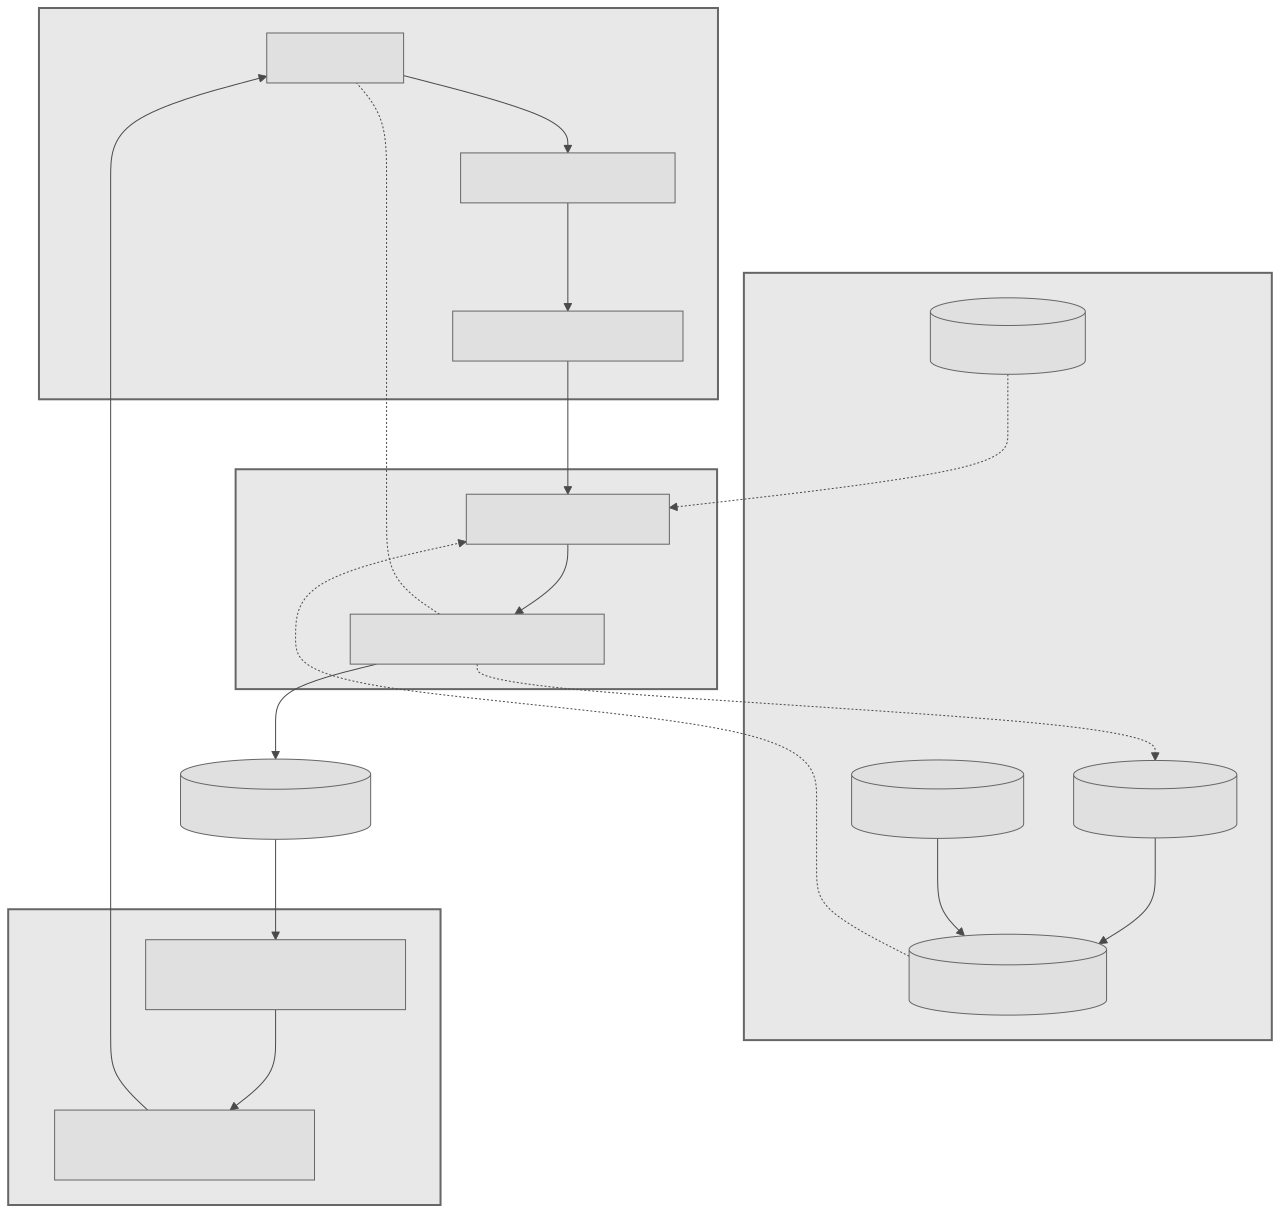
\includegraphics[width=0.95\textwidth,height=\textheight]{figures/architecture.mmd.png}
\caption{Healthcare Analytics Architecture. Solid lines indicate the
primary data flow from clinical user natural language queries through a
conversational AI interface to a healthcare NLP engine for context-aware
SQL generation. Bi-directional arrows at steps 5 and 8 represent the
iterative `Query \& Refine' loop where users refine their intent based
on delivered insights. The critical validation step (dotted
bi-directional line) shows domain experts confirming or correcting
generated SQL before results are trusted. Validated NL-SQL-Rationale
triples flow to organizational memory (dashed line), where they persist
independent of staff tenure and inform future query generation.}
\end{figure}

\begin{figure}
\centering
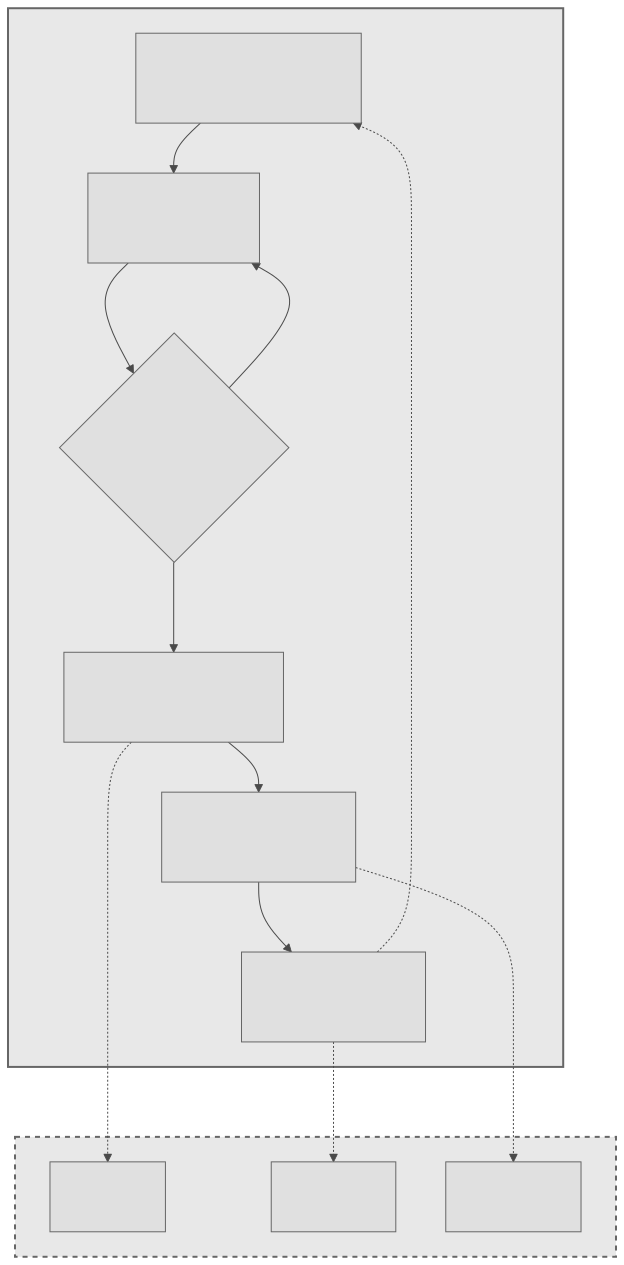
\includegraphics[width=0.5\textwidth,height=\textheight]{figures/knowledge-cycle.mmd.png}
\caption{The Validated Query Cycle, shown as six numbered steps in the
diagram. (1) Domain experts ask natural language questions, (2) the
system generates candidate SQL, (3) AI provides a natural language
explanation of the SQL logic; domain expert confirms the intent and
results, (4) validated triples are stored, (5) future queries retrieve
validated knowledge, and (6) expertise persists through staff turnover.
This cycle breaks the compounding effect where turnover erases
institutional memory.}
\end{figure}

\section{Discussion}\label{discussion}

\subsection{Market Barriers and Standardization
Failure}\label{market-barriers-and-standardization-failure}

Efforts to standardize healthcare analytics often fail due to the
tension between local clinical reality and centralized models.
High-profile industry events illustrate these documented challenges. IBM
divested its Watson Health data and analytics assets to Francisco
Partners in 2022 (\citeproc{ref-ibm2022}{110}), following years of
underperformance attributed to a fundamental mismatch between AI
capabilities and clinical reality: the technology encountered the
``messy reality'' of healthcare data environments where centralized
models failed to account for the highly variable, institution-specific
business logic embedded in clinical workflows
(\citeproc{ref-strickland2019}{111},\citeproc{ref-yang2020}{112}).
Academic analysis identified additional contributing factors including
suboptimal business performance (only breaking even), a restrictive
top-down commercialization strategy that limited market reach, and the
highly-regulated nature of healthcare creating barriers to AI deployment
(\citeproc{ref-yang2020}{112}). The Haven healthcare venture (backed by
Amazon, Berkshire Hathaway, and JPMorgan Chase) disbanded in 2021 after
three years (\citeproc{ref-lavito2021}{113}), with academic analysis
identifying multiple contributing factors: even the three founding
companies could not effectively share health-care cost data with each
other, the venture never employed more than 75 people (limiting its
ability to effect industry-wide change), and leadership turnover
destabilized organizational continuity
(\citeproc{ref-acchiardo2021}{114}). Research on Big Tech platform entry
into healthcare positions both Watson Health and Haven within a broader
pattern of technology companies encountering regulatory complexity and
institutional resistance when attempting to standardize fragmented
healthcare systems (\citeproc{ref-ozalp2022}{115}). These outcomes align
with the academic literature's findings: standardized solutions face
significant barriers when applied across institutions with unique data
definitions, business rules, and clinical workflows.

\subsection{The Validator Paradox and Knowledge
Ratchet}\label{the-validator-paradox-and-knowledge-ratchet}

A critical paradox exists: if experts are leaving (Pillar 2), who
validates the AI (Pillar 3)? We resolve this via the concept of the
``organizational knowledge ratchet'' (\citeproc{ref-rao2006}{61}).
Validation must be reframed not as \emph{eternal truth} but as the
``standard work'' of informatics, drawing on Lean management principles
(\citeproc{ref-alukal2006}{116}).

In this model, a validated query represents the ``current best way'' to
perform an analysis. As Alukal and Manos
(\citeproc{ref-alukal2006}{116}) establish, standard work is the
prerequisite for Kaizen (continuous improvement): without a documented
standard, there is no baseline to improve upon. Even provisional
validation by mid-level analysts captures operational logic into a
durable artifact. This prevents the ``sliding back to zero''
characteristic of high-turnover environments
(\citeproc{ref-hong2025}{75}). Rather than requiring a permanent core of
experts, the system accumulates knowledge incrementally, using the
structure of the validation process to buffer against the disruptive
effects of turnover.

\subsection{Lifecycle Management: Continuous Analytic
Integration}\label{lifecycle-management-continuous-analytic-integration}

Leveraging the property of Executability, a validated SQL query is
treated not as a static artifact but as a software asset within a CI/CD
pipeline. In healthcare, database schemas (Epic, Cerner, OMOP) change
frequently, breaking ``frozen'' code. To address ``Schema Drift,''
analytics must adopt principles from software engineering:
\emph{Continuous Analytic Integration}. In this approach, Validated
Query Triples are managed not as wiki entries but as software assets
within a CI/CD pipeline. When the data warehouse schema is updated
(e.g., a quarterly EHR upgrade), the system automatically re-runs the
library of stored queries. Queries that fail or return anomalous results
are flagged for review. This transforms ``Institutional Memory'' from a
stagnant repository into a living, automated test suite that actively
signals when organizational knowledge has drifted from technical
reality.

\subsection{Mitigating ``Shadow IT'' with ``Golden
Queries''}\label{mitigating-shadow-it-with-golden-queries}

To prevent the ``chaos of conflicting definitions'' that can arise from
democratized analytics, organizations can introduce a ``Golden Query''
governance status. In this model, a central committee can certify
specific validated triples as the ``source of truth'' for the
organization (\citeproc{ref-himss2025ucdavis}{117}). This ensures that
while many users can create and validate queries, only a select few are
designated as the official, trusted queries for key metrics, thus
mitigating the risks of ``Shadow IT''
(\citeproc{ref-zimmermann2017}{118}).

\subsection{Economic and Strategic
Implications}\label{economic-and-strategic-implications}

The economic case for intervention is supported by evidence linking
conversational analytics to a 206\% three-year ROI and reduced
development times
(\citeproc{ref-forrester2024}{28},\citeproc{ref-elkamouchi2023}{119}--\citeproc{ref-precedence2024}{122}).
Low-code and AI platforms democratize access, allowing organizations to
achieve ``Shadow IT'' agility within a governed framework
(\citeproc{ref-himss2025ucdavis}{117},\citeproc{ref-zimmermann2017}{118},\citeproc{ref-rivard1987}{123},\citeproc{ref-kopper2020}{124}).
Other benefits include faster revenue cycles
(\citeproc{ref-pennington2023}{125}) and cost reductions
(\citeproc{ref-jiao2023}{126}--\citeproc{ref-forrester2024a}{129}).

\subsection{Limitations and Future
Research}\label{limitations-and-future-research}

This review is limited by its narrative design and the rapid evolution
of the field. Evidence gaps remain regarding long-term outcomes
(\citeproc{ref-sezgin2022}{130}), specialty-specific applications, and
governance frameworks for democratized analytics. Future research should
prioritize: (1) validation of NL2SQL on synthetic healthcare data (e.g.,
Synthea), (2) automated schema discovery algorithms, and (3)
longitudinal studies of organizational transformation.

\section{Conclusion}\label{conclusion}

We developed a three-pillar analytical framework connecting analytics
maturity, workforce agility, and technical enablement. The evidence
reveals that these challenges are self-reinforcing: low maturity
accelerates turnover, turnover degrades the institutional memory needed
for maturity, and technical barriers prevent knowledge capture.

By deploying technical enablement, specifically conversational AI with a
validated query cycle, organizations can break this cycle. This approach
captures tacit knowledge as executable artifacts, ensuring that
expertise persists independently of individual staff tenure. Applying
the principle of \emph{primum non nocere}, healthcare leaders must
recognize that inaction in the face of workforce instability allows the
continued degradation of organizational capability.

\section{Acknowledgments}\label{acknowledgments}

The author (S.T.H.) takes full responsibility for the final content.
Gemini CLI (Gemini 3, Google) assisted with manuscript editing and
refinement. The author takes full responsibility for the final content.

\section{Funding}\label{funding}

Yuimedi provided funding for the author's time writing and researching
this manuscript.

\section{Abbreviations}\label{abbreviations}

AACODS: Authority, Accuracy, Coverage, Objectivity, Date, Significance
AI: Artificial Intelligence AMAM: Analytics Maturity Assessment Model
CIO: Chief Information Officer DIKW: Data-Information-Knowledge-Wisdom
EHR: Electronic Health Record EMRAM: Electronic Medical Record Adoption
Model HIMSS: Healthcare Information Management Systems Society IT:
Information Technology NL2SQL: Natural Language to SQL NLP: Natural
Language Processing SQL: Structured Query Language

\section{Author Contributions}\label{author-contributions}

S.T.H. conceived the research, conducted the literature review, and
wrote the manuscript.

\section{Conflicts of Interest}\label{conflicts-of-interest}

The author is a contract product advisor at Yuimedi, Inc.~and employed
at Indiana University Health. The views expressed are the author's own.

\section{Data Availability}\label{data-availability}

This is a narrative review; no primary datasets were generated.

\section{References}\label{references}

\phantomsection\label{refs}
\begin{CSLReferences}{0}{1}
\bibitem[\citeproctext]{ref-american2023}
\CSLLeftMargin{1. }%
\CSLRightInline{NORC at the University of Chicago AHIMA \&. {Health
information workforce survey report} {[}Internet{]}. American Health
Information Management Association \& {NORC} at the University of
Chicago; 2023. Available from:
\url{https://www.ahima.org/news-publications/press-room-press-releases/2023-press-releases/health-information-workforce-shortages-persist-as-ai-shows-promise-ahima-survey-reveals/}}

\bibitem[\citeproctext]{ref-himss2024}
\CSLLeftMargin{2. }%
\CSLRightInline{Analytics H. {Analytics maturity assessment model (AMAM)
global report. Healthcare Information and Management Systems Society}
{[}Internet{]}. {HIMSS} Analytics; 2024. Available from:
\url{https://www.himss.org/maturity-models/amam/}}

\bibitem[\citeproctext]{ref-himss2024news}
\CSLLeftMargin{3. }%
\CSLRightInline{Healthcare IT News. {HIMSS launches modernised Analytics
Maturity Assessment Model} {[}Internet{]}. 2024. Available from:
\url{https://www.healthcareitnews.com/news/asia/himss24-apac-adoption-model-analytics-maturity-gets-facelift}}

\bibitem[\citeproctext]{ref-wittkieffer2024}
\CSLLeftMargin{4. }%
\CSLRightInline{WittKieffer. {CIO Insights: The State of Healthcare IT
Leadership} {[}Internet{]}. WittKieffer; 2024. Available from:
\url{https://api.wittkieffer.com/wp-content/uploads/2012/10/cio-insights-the-state-of-healthcare-it-leadership-wittkieffer-october-2024.pdf}}

\bibitem[\citeproctext]{ref-himssworkforce2024}
\CSLLeftMargin{5. }%
\CSLRightInline{HIMSS. {The Future of Workforce} {[}Internet{]}.
Healthcare Information; Management Systems Society; 2024. Available
from: \url{https://www.himss.org/resources/the-future-of-workforce/}}

\bibitem[\citeproctext]{ref-rajamani2025}
\CSLLeftMargin{6. }%
\CSLRightInline{Rajamani L S. {Public health informatics specialists in
state and local public health workforce: Insights from public health
workforce interests and needs survey}. Journal of Public Health
Management and Practice {[}Internet{]}. 2025; Available from:
\url{https://academic.oup.com/jpubhealth}}

\bibitem[\citeproctext]{ref-gal2019}
\CSLLeftMargin{7. }%
\CSLRightInline{Gal MS, Rubinfeld DL. {Data Standardization}. NYU Law
Review {[}Internet{]}. 2019;94(4):737--70. Available from:
\url{https://www.nyulawreview.org/issues/volume-94-number-4/data-standardization/}}

\bibitem[\citeproctext]{ref-zhang2024}
\CSLLeftMargin{8. }%
\CSLRightInline{Zhang Y, Callaghan-Koru JA, Koru G. {The challenges and
opportunities of continuous data quality improvement for healthcare
administration data}. JAMIA Open. 2024;7(2):ooae042. }

\bibitem[\citeproctext]{ref-rowley2007}
\CSLLeftMargin{9. }%
\CSLRightInline{Rowley J.
\href{https://doi.org/10.1177/0165551506070706}{{The wisdom hierarchy:
representations of the DIKW hierarchy}}. Journal of Information Science.
2007;33(2):163--80. }

\bibitem[\citeproctext]{ref-massingham2018}
\CSLLeftMargin{10. }%
\CSLRightInline{Massingham PR. {Measuring the impact of knowledge loss:
A longitudinal study}. Journal of Knowledge Management {[}Internet{]}.
2018; Available from: \url{https://doi.org/10.1108/JKM-08-2016-0338}}

\bibitem[\citeproctext]{ref-farnese2019}
\CSLLeftMargin{11. }%
\CSLRightInline{Farnese B M. L. {Managing knowledge in organizations: A
Nonaka's {SECI} model operationalization}. Frontiers in Psychology
{[}Internet{]}. 2019; Available from:
\url{https://www.frontiersin.org/articles/10.3389/fpsyg.2019.02730}}

\bibitem[\citeproctext]{ref-foos2006}
\CSLLeftMargin{12. }%
\CSLRightInline{Foos S T. {Tacit knowledge transfer and the knowledge
disconnect}. Journal of Knowledge Management {[}Internet{]}. 2006;
Available from:
\url{https://www.emerald.com/insight/content/doi/10.1108/13673270610650067/full/html}}

\bibitem[\citeproctext]{ref-benbya2004}
\CSLLeftMargin{13. }%
\CSLRightInline{Benbya P H. {Corporate portal: A tool for knowledge
management synchronization}. International Journal of Information
Management {[}Internet{]}. 2004; Available from:
\url{https://doi.org/10.1016/j.ijinfomgt.2003.12.012}}

\bibitem[\citeproctext]{ref-zhang2025}
\CSLLeftMargin{14. }%
\CSLRightInline{Zhang D W. {{AI} challenges conventional knowledge
management: Light the way for reframing {SECI} model and Ba theory}.
Journal of Knowledge Management {[}Internet{]}. 2025; Available from:
\url{https://www.emerald.com/insight/content/doi/10.1108/JKM-03-2024-0262/full/html}}

\bibitem[\citeproctext]{ref-allison2021}
\CSLLeftMargin{15. }%
\CSLRightInline{Allison DG, Peters H. {Root Cause Analysis (RCA) for the
Improvement of Healthcare Systems and Patient Safety} {[}Internet{]}.
CRC Press; 2021. Available from:
\url{https://doi.org/10.1201/9781003188162}}

\bibitem[\citeproctext]{ref-soylemez2017}
\CSLLeftMargin{16. }%
\CSLRightInline{Soylemez M, Tarhan A. {A Review and Comparison of
Maturity/Capability Frameworks for Healthcare Process Assessment and
Improvement}. Software Quality Professional {[}Internet{]}.
2017;19:28--42. Available from:
\url{https://openurl.ebsco.com/EPDB\%3Agcd\%3A3\%3A34056963/detailv2?sid=ebsco\%3Aplink\%3Ascholar&id=ebsco\%3Agcd\%3A121526814}}

\bibitem[\citeproctext]{ref-latrella2024}
\CSLLeftMargin{17. }%
\CSLRightInline{Latrella \&B M. {Improving patient outcomes while
reducing readmissions with data analytics}. Management in Healthcare
{[}Internet{]}. 2024; Available from:
\url{https://www.ingentaconnect.com/content/hsp/mih/2024/00000008/00000004/art00006}}

\bibitem[\citeproctext]{ref-nashid2023}
\CSLLeftMargin{18. }%
\CSLRightInline{Nashid P S., Hossain MI. {Advanced Business Analytics in
Healthcare: Enhancing Clinical Decision Support and Operational
Efficiency}. Business and Social Sciences {[}Internet{]}.
2023;1(1):1--8. Available from:
\url{https://doi.org/10.25163/business.1110345}}

\bibitem[\citeproctext]{ref-shahbaz2019}
\CSLLeftMargin{19. }%
\CSLRightInline{Shahbaz G M. {Investigating the adoption of big data
analytics in healthcare: The moderating role of resistance to change}.
Journal of Big Data {[}Internet{]}. 2019; Available from:
\url{https://journalofbigdata.springeropen.com/articles/10.1186/s40537-019-0170-y}}

\bibitem[\citeproctext]{ref-kamble2019}
\CSLLeftMargin{20. }%
\CSLRightInline{Kamble G S. S. {A systematic perspective on the
applications of big data analytics in healthcare management}.
International Journal of Healthcare Management {[}Internet{]}. 2019;
Available from:
\url{https://www.tandfonline.com/doi/full/10.1080/20479700.2018.1531606}}

\bibitem[\citeproctext]{ref-ziletti2024}
\CSLLeftMargin{21. }%
\CSLRightInline{Ziletti \&D A. {Retrieval augmented text-to-SQL
generation for epidemiological question answering using electronic
health records}. {NAACL} 2024 Clinical {NLP} Workshop {[}Internet{]}.
2024; Available from: \url{https://arxiv.org/abs/2403.09226}}

\bibitem[\citeproctext]{ref-wang2025}
\CSLLeftMargin{22. }%
\CSLRightInline{Wang H S. {Capabilities of GPT-5 on multimodal medical
reasoning}. arXiv preprint {[}Internet{]}. 2025; Available from:
\url{https://arxiv.org/abs/2508.08224}}

\bibitem[\citeproctext]{ref-tyndall2010}
\CSLLeftMargin{23. }%
\CSLRightInline{Tyndall J. {{AACODS} Checklist. Flinders University}
{[}Internet{]}. 2010. Available from:
\url{https://dspace.flinders.edu.au/jspui/bitstream/2328/3326/4/AACODS_Checklist.pdf}}

\bibitem[\citeproctext]{ref-berkshire2024}
\CSLLeftMargin{24. }%
\CSLRightInline{Trust BHN. {Empowering citizen developers: Low-code
success in healthcare} {[}Internet{]}. 2024. Available from:
\url{https://ia.berkshirehealthcare.nhs.uk/citizen-developer-programme}}

\bibitem[\citeproctext]{ref-snowdon2024b}
\CSLLeftMargin{25. }%
\CSLRightInline{Snowdon A. {New analytics maturity adoption model pushes
for digital transformation and data-driven decisions}. {HIMSS}
{[}Internet{]}. 2024; Available from:
\url{https://legacy.himss.org/news/new-analytics-maturity-adoption-model-pushes-digital-transformation-and-data-driven-decisions}}

\bibitem[\citeproctext]{ref-oracle2024}
\CSLLeftMargin{26. }%
\CSLRightInline{Oracle. {The real cost of turnover in healthcare}
{[}Internet{]}. 2024. Available from:
\url{https://www.oracle.com/human-capital-management/cost-employee-turnover-healthcare/}}

\bibitem[\citeproctext]{ref-health2020}
\CSLLeftMargin{27. }%
\CSLRightInline{Catalyst H. {The healthcare analytics adoption model: A
roadmap to analytic maturity} {[}Internet{]}. 2020. Available from:
\url{https://www.healthcatalyst.com/learn/insights/healthcare-analytics-adoption-model-roadmap-analytic-maturity}}

\bibitem[\citeproctext]{ref-forrester2024}
\CSLLeftMargin{28. }%
\CSLRightInline{Research F. {The total economic impact of Microsoft
Power Apps. Forrester Consulting} {[}Internet{]}. 2024. Available from:
\url{https://tei.forrester.com/go/microsoft/powerappstei/?lang=en-us}}

\bibitem[\citeproctext]{ref-wang2018}
\CSLLeftMargin{29. }%
\CSLRightInline{Wang K Y., Byrd TA. {Big data analytics: Understanding
its capabilities and potential benefits for healthcare organizations}.
Technological Forecasting and Social Change {[}Internet{]}.
2018;126:3--13. Available from:
\url{https://www.sciencedirect.com/science/article/abs/pii/S0040162516000500}}

\bibitem[\citeproctext]{ref-wang2017}
\CSLLeftMargin{30. }%
\CSLRightInline{Wang \&H Y. {Exploring the path to big data analytics
success in healthcare}. Journal of Business Research {[}Internet{]}.
2017; Available from:
\url{https://www.sciencedirect.com/science/article/abs/pii/S0148296316304891}}

\bibitem[\citeproctext]{ref-tgh2025}
\CSLLeftMargin{31. }%
\CSLRightInline{Tampa General Hospital. {Tampa General Hospital Awarded
Highest Designation in Analytics by HIMSS} {[}Internet{]}. 2025.
Available from:
\url{https://www.tgh.org/news/tgh-press-releases/2025/june/tampa-general-hospital-awarded-highest-designation-analytics-himss}}

\bibitem[\citeproctext]{ref-cmuh2025}
\CSLLeftMargin{32. }%
\CSLRightInline{China Medical University Hospital. {Taiwan's First
Hospital to Achieve AMAM Stage 7 Certification!} {[}Internet{]}. PR
Newswire; 2025. Available from:
\url{https://www.prnewswire.com/news-releases/taiwans-first-hospital-to-achieve-amam-stage-7-certification-302390824.html}}

\bibitem[\citeproctext]{ref-ksa2024}
\CSLLeftMargin{33. }%
\CSLRightInline{Medical Buyer. {2 medical groups in Saudi Arabia achieve
stage 7 digital maturity} {[}Internet{]}. 2024. Available from:
\url{https://medicalbuyer.co.in/2-medical-groups-in-saudi-arabia-achieve-stage-7-digital-maturity/}}

\bibitem[\citeproctext]{ref-himss2024apac}
\CSLLeftMargin{34. }%
\CSLRightInline{Healthcare IT News. {At HIMSS24 APAC, the Adoption Model
for Analytics Maturity gets facelift} {[}Internet{]}. 2024. Available
from:
\url{https://www.healthcareitnews.com/news/asia/himss24-apac-adoption-model-analytics-maturity-gets-facelift}}

\bibitem[\citeproctext]{ref-snowdon2024}
\CSLLeftMargin{35. }%
\CSLRightInline{Snowdon H A., Wright A. {Digital maturity as a predictor
of quality and safety outcomes in {US} hospitals: Cross-sectional
observational study}. Journal of Medical Internet Research
{[}Internet{]}. 2024;26:e56316. Available from:
\url{https://www.jmir.org/2024/1/e56316}}

\bibitem[\citeproctext]{ref-snowdon2024a}
\CSLLeftMargin{36. }%
\CSLRightInline{Snowdon H A. {Digital maturity as a strategy for
advancing patient experience in {US} hospitals}. Journal of Patient
Experience {[}Internet{]}. 2024; Available from:
\url{https://journals.sagepub.com/doi/full/10.1177/23743735241253785}}

\bibitem[\citeproctext]{ref-wang2019}
\CSLLeftMargin{37. }%
\CSLRightInline{Wang K Y. {Leveraging big data analytics to improve
quality of care in healthcare organizations: A configurational
perspective}. British Journal of Management {[}Internet{]}. 2019;
Available from:
\url{https://onlinelibrary.wiley.com/doi/abs/10.1111/1467-8551.12332}}

\bibitem[\citeproctext]{ref-gomes2025}
\CSLLeftMargin{38. }%
\CSLRightInline{Gomes \&R J. {Evaluating maturity models in healthcare
information systems: A comprehensive review}. Healthcare {[}Internet{]}.
2025; Available from: \url{https://www.mdpi.com/2227-9032/13/1/1}}

\bibitem[\citeproctext]{ref-woods2024}
\CSLLeftMargin{39. }%
\CSLRightInline{Woods L, Eden R, Green D, Pearce A. {Impact of digital
health on the quadruple aims of healthcare: A correlational and
longitudinal study (Digimat Study)}. International Journal of Medical
Informatics {[}Internet{]}. 2024; Available from:
\url{https://www.sciencedirect.com/science/article/pii/S1386505624001916}}

\bibitem[\citeproctext]{ref-martin2019}
\CSLLeftMargin{40. }%
\CSLRightInline{Martin G, Clarke J, Liew F, Arora S, King D, Aylin P.
{Evaluating the impact of organisational digital maturity on clinical
outcomes in secondary care in England}. npj Digital Medicine
{[}Internet{]}. 2019; Available from:
\url{https://www.nature.com/articles/s41746-019-0118-9}}

\bibitem[\citeproctext]{ref-saintulysse2021}
\CSLLeftMargin{41. }%
\CSLRightInline{Saint-Ulysse C. {The Relationship between Hospitals'
Electronic Health Records Maturity and Excess Readmission Ratio}
{[}Internet{]}. Walden University Dissertations; 2021. Available from:
\url{https://scholarworks.waldenu.edu/cgi/viewcontent.cgi?article=12395&context=dissertations}}

\bibitem[\citeproctext]{ref-yang2021}
\CSLLeftMargin{42. }%
\CSLRightInline{Yang DX, Khera R, Miccio JA, Jairam V, et al.
{Prevalence of missing data in the national cancer database and
association with overall survival}. JAMA Network Open {[}Internet{]}.
2021;4(3):e211793. Available from:
\url{https://jamanetwork.com/journals/jamanetworkopen/fullarticle/2777777}}

\bibitem[\citeproctext]{ref-arts2002}
\CSLLeftMargin{43. }%
\CSLRightInline{Arts DG, De Keizer NF, et al. {Defining and improving
data quality in medical registries: a literature review, case study, and
generic framework}. Journal of the American Medical Informatics
Association {[}Internet{]}. 2002;9(6):600--11. Available from:
\url{https://academic.oup.com/jamia/article-abstract/9/6/600/1036696}}

\bibitem[\citeproctext]{ref-mccoy2013}
\CSLLeftMargin{44. }%
\CSLRightInline{McCoy AB, Wright A, Kahn MG, Shapiro JS, et al.
{Matching identifiers in electronic health records: implications for
duplicate records and patient safety}. BMJ Quality \& Safety
{[}Internet{]}. 2013;22(3):219--24. Available from:
\url{https://qualitysafety.bmj.com/content/22/3/219.short}}

\bibitem[\citeproctext]{ref-rahman2020}
\CSLLeftMargin{45. }%
\CSLRightInline{Rahman P, Nandi A, Hebert C. {Amplifying domain
expertise in clinical data pipelines}. JMIR Medical Informatics
{[}Internet{]}. 2020;8(11):e19612. Available from:
\url{https://medinform.jmir.org/2020/11/e19612/}}

\bibitem[\citeproctext]{ref-sirgo2018}
\CSLLeftMargin{46. }%
\CSLRightInline{Sirgo G, Esteban G Francisco icon, Moreno G, et al.
{Validation of the ICU-DaMa tool for automatically extracting variables
for minimum dataset and quality indicators: The importance of data
quality assessment}. International Journal of Medical Informatics
{[}Internet{]}. 2018;112:166--72. Available from:
\url{https://www.sciencedirect.com/science/article/abs/pii/S1386505618300443}}

\bibitem[\citeproctext]{ref-shi2021}
\CSLLeftMargin{47. }%
\CSLRightInline{Shi X, Prins C, Van Pottelbergh G, Mamouris P, et al.
{An automated data cleaning method for Electronic Health Records by
incorporating clinical knowledge}. BMC Medical Informatics and Decision
Making {[}Internet{]}. 2021;21:1--12. Available from:
\url{https://link.springer.com/article/10.1186/s12911-021-01470-5}}

\bibitem[\citeproctext]{ref-dugas2016}
\CSLLeftMargin{48. }%
\CSLRightInline{Dugas M, Neuhaus P, Meidt A, Doods J, Storck M, et al.
{Portal of medical data models: information infrastructure for medical
research and healthcare}. Database {[}Internet{]}. 2016;2016. Available
from:
\url{https://academic.oup.com/database/article/doi/10.1093/database/bav121/2630096}}

\bibitem[\citeproctext]{ref-bokov2017}
\CSLLeftMargin{49. }%
\CSLRightInline{Bokov AF, Bos AB, Manuel LS, et al. {Using prevalence
patterns to discover un-mapped flowsheet data in an electronic health
record data warehouse}. In: 2017 IEEE 30th international symposium on
computer-based medical systems (CBMS) {[}Internet{]}. IEEE; 2017. p.
509--14. Available from:
\url{https://ieeexplore.ieee.org/abstract/document/8104211}}

\bibitem[\citeproctext]{ref-ulrich2022}
\CSLLeftMargin{50. }%
\CSLRightInline{Ulrich H, Kock-Schoppenhauer AK, et al. {Understanding
the nature of metadata: systematic review}. Journal of Medical Internet
Research {[}Internet{]}. 2022;24(1):e25440. Available from:
\url{https://www.jmir.org/2022/1/e25440/}}

\bibitem[\citeproctext]{ref-lucyk2017}
\CSLLeftMargin{51. }%
\CSLRightInline{Lucyk K, Tang K, Quan H. {Barriers to data quality
resulting from the process of coding health information to
administrative data: a qualitative study}. BMC Health Services Research
{[}Internet{]}. 2017;17(1):1--10. Available from:
\url{https://link.springer.com/article/10.1186/s12913-017-2697-y}}

\bibitem[\citeproctext]{ref-hovenga2013}
\CSLLeftMargin{52. }%
\CSLRightInline{Hovenga EJ, Grain H. {Health data and data governance}.
In: Health information governance in a digital environment
{[}Internet{]}. IOS Press; 2013. p. 67--94. Available from:
\url{https://ebooks.iospress.nl/volumearticle/35106}}

\bibitem[\citeproctext]{ref-carvalho2019}
\CSLLeftMargin{53. }%
\CSLRightInline{Carvalho JV, Rocha Á, Vasconcelos J.
\href{https://doi.org/10.1016/j.ijinfomgt.2018.07.001}{{A health data
analytics maturity model for hospitals information systems}}.
International Journal of Information Management. 2019;46:278--85. }

\bibitem[\citeproctext]{ref-pintovalverde2013}
\CSLLeftMargin{54. }%
\CSLRightInline{Pinto-Valverde J, Pérez-Guardado M. {HDQM2: healthcare
data quality maturity model}. In: Midwest association for information
systems conference {[}Internet{]}. 2013. Available from:
\url{https://scholarworks.wmich.edu/ichita_transactions/37/}}

\bibitem[\citeproctext]{ref-gokalp2023}
\CSLLeftMargin{55. }%
\CSLRightInline{G"okalp MO, G"okalp E, G"okalp S. {The development of
data analytics maturity assessment framework: DAMAF}. Journal of
Software: Evolution and Process {[}Internet{]}. 2023;35(4):e2448.
Available from:
\url{https://onlinelibrary.wiley.com/doi/abs/10.1002/smr.2415}}

\bibitem[\citeproctext]{ref-lismont2017}
\CSLLeftMargin{56. }%
\CSLRightInline{Lismont J, Vanthienen J, Baesens B, et al. {Defining
analytics maturity indicators: A survey approach}. International Journal
of Information Management {[}Internet{]}. 2017;37(3):114--24. Available
from:
\url{https://www.sciencedirect.com/science/article/abs/pii/S0268401216305655}}

\bibitem[\citeproctext]{ref-ang2004}
\CSLLeftMargin{57. }%
\CSLRightInline{Ang \&S S. {Turnover of information technology
professionals: The effects of internal labor market strategies}. {ACM}
{SIGMIS} Database: The {DATABASE} for Advances in Information Systems
{[}Internet{]}. 2004; Available from:
\url{https://dl.acm.org/doi/10.1145/1017114.1017118}}

\bibitem[\citeproctext]{ref-wu2024}
\CSLLeftMargin{58. }%
\CSLRightInline{Wu L F., Li L. {Worldwide prevalence and associated
factors of nursing staff turnover: A systematic review and
meta-analysis}. Nursing Open {[}Internet{]}. 2024;11:e2097. Available
from: \url{https://pmc.ncbi.nlm.nih.gov/articles/PMC10802134/}}

\bibitem[\citeproctext]{ref-ren2024}
\CSLLeftMargin{59. }%
\CSLRightInline{Ren W L. {Global prevalence of nurse turnover rates: A
meta-analysis of 21 studies from 14 countries}. Journal of Nursing
Management {[}Internet{]}. 2024; Available from:
\url{https://pmc.ncbi.nlm.nih.gov/articles/PMC11919231/}}

\bibitem[\citeproctext]{ref-willardgrace2019}
\CSLLeftMargin{60. }%
\CSLRightInline{Willard-Grace K R. {Burnout and health care workforce
turnover}. The Annals of Family Medicine {[}Internet{]}. 2019; Available
from: \url{https://www.annfammed.org/content/17/1/36}}

\bibitem[\citeproctext]{ref-rao2006}
\CSLLeftMargin{61. }%
\CSLRightInline{Rao RD, Argote L. Organizational learning and
forgetting: The effects of turnover and structure. European Management
Review {[}Internet{]}. 2006;3(2):77--85. Available from:
\url{https://onlinelibrary.wiley.com/doi/abs/10.1057/palgrave.emr.1500057}}

\bibitem[\citeproctext]{ref-mayo2016}
\CSLLeftMargin{62. }%
\CSLRightInline{Mayo D C. S. {How can we effect culture change toward
data-driven medicine?} International Journal of Radiation Oncology,
Biology, Physics {[}Internet{]}. 2016; Available from:
\url{https://www.redjournal.org/article/S0360-3016(16)00260-1/fulltext}}

\bibitem[\citeproctext]{ref-goffin2011}
\CSLLeftMargin{63. }%
\CSLRightInline{Goffin \&K K. {Tacit knowledge, lessons learnt, and new
product development}. Journal of Product Innovation Management
{[}Internet{]}. 2011; Available from:
\url{https://onlinelibrary.wiley.com/doi/abs/10.1111/j.1540-5885.2010.00798.x}}

\bibitem[\citeproctext]{ref-ledikwe2013}
\CSLLeftMargin{64. }%
\CSLRightInline{Ledikwe R J. H. {Establishing a health information
workforce: Innovation for low- and middle-income countries}. Human
Resources for Health {[}Internet{]}. 2013; Available from:
\url{https://human-resources-health.biomedcentral.com/articles/10.1186/1478-4491-11-35}}

\bibitem[\citeproctext]{ref-mantas2010}
\CSLLeftMargin{65. }%
\CSLRightInline{Mantas A J. {Recommendations of the International
Medical Informatics Association (IMIA) on education in biomedical and
health informatics: First revision}. Methods of Information in Medicine
{[}Internet{]}. 2010; Available from:
\url{https://pubmed.ncbi.nlm.nih.gov/20054502/}}

\bibitem[\citeproctext]{ref-musa2023}
\CSLLeftMargin{66. }%
\CSLRightInline{Musa D S. {The impact of training on electronic health
records related knowledge, practical competencies, and staff
satisfaction: A pre-post intervention study among wellness center
providers in a primary health-care facility}. Journal of
Multidisciplinary Healthcare {[}Internet{]}. 2023; Available from:
\url{https://pmc.ncbi.nlm.nih.gov/articles/PMC10243608/}}

\bibitem[\citeproctext]{ref-konrad2022}
\CSLLeftMargin{67. }%
\CSLRightInline{Konrad \&S I. {Exploring the potential of an {IT}
capability in its bootstrap phase from a task driven onboarding
perspective: Insights toward information infrastructure in healthcare}
{[}Internet{]} {[}Master's thesis{]}. 2022. Available from:
\url{https://www.diva-portal.org/smash/record.jsf?pid=diva2:1684142}}

\bibitem[\citeproctext]{ref-wang2020}
\CSLLeftMargin{68. }%
\CSLRightInline{Wang S P. {Text-to-SQL generation for question answering
on electronic medical records}. In: Proceedings of the web conference
2020 {[}Internet{]}. 2020. Available from:
\url{https://arxiv.org/abs/1908.01839}}

\bibitem[\citeproctext]{ref-goffin2010}
\CSLLeftMargin{69. }%
\CSLRightInline{Goffin K K. {Managing lessons learned and tacit
knowledge in new product development}. Research-Technology Management
{[}Internet{]}. 2010; Available from:
\url{https://www.tandfonline.com/doi/abs/10.1080/08956308.2010.11657637}}

\bibitem[\citeproctext]{ref-rintala2006}
\CSLLeftMargin{70. }%
\CSLRightInline{Rintala \&H N. {Methods for sharing tacit nuclear
knowledge and expertise}. International Journal of Nuclear Knowledge
Management {[}Internet{]}. 2006; Available from:
\url{https://www.inderscienceonline.com/doi/abs/10.1504/IJNKM.2006.009880}}

\bibitem[\citeproctext]{ref-bardsley2016}
\CSLLeftMargin{71. }%
\CSLRightInline{Bardsley M. {Understanding analytical capability in
health care: Do we have more data than insight? The Health Foundation}
{[}Internet{]}. 2016. Available from:
\url{https://www.health.org.uk/publications/understanding-analytical-capability-in-health-care}}

\bibitem[\citeproctext]{ref-yuan2019}
\CSLLeftMargin{72. }%
\CSLRightInline{Yuan R C. {Criteria2Query: a natural language interface
to clinical databases for cohort definition}. Journal of the American
Medical Informatics Association {[}Internet{]}. 2019; Available from:
\url{https://academic.oup.com/jamia/article-abstract/26/4/294/5308980}}

\bibitem[\citeproctext]{ref-pesqueira2020}
\CSLLeftMargin{73. }%
\CSLRightInline{Pesqueira S A. {Big data skills sustainable development
in healthcare and pharmaceuticals}. Journal of Medical Systems
{[}Internet{]}. 2020; Available from:
\url{https://link.springer.com/article/10.1007/s10916-020-01665-9}}

\bibitem[\citeproctext]{ref-nsi2025}
\CSLLeftMargin{74. }%
\CSLRightInline{NSI Nursing Solutions. {2025 National Health Care
Retention \& RN Staffing Report} {[}Internet{]}. NSI Nursing Solutions;
2024. Available from:
\url{https://www.nsinursingsolutions.com/documents/library/nsi_national_health_care_retention_report.pdf}}

\bibitem[\citeproctext]{ref-hong2025}
\CSLLeftMargin{75. }%
\CSLRightInline{Hong JH. When does employee turnover matter?
Organizational memory in federal IT. Journal of Public Administration
Research and Theory {[}Internet{]}. 2025; Available from:
\url{https://academic.oup.com/jpart/advance-article-abstract/doi/10.1093/jopart/muaf019/8162522}}

\bibitem[\citeproctext]{ref-openai2025}
\CSLLeftMargin{76. }%
\CSLRightInline{OpenAI. {HealthBench: A benchmark for evaluating LLMs in
healthcare}. arXiv preprint {[}Internet{]}. 2025; Available from:
\url{https://arxiv.org/abs/2505.08775}}

\bibitem[\citeproctext]{ref-wu2024a}
\CSLLeftMargin{77. }%
\CSLRightInline{Wu Q C., Xie W. {Towards evaluating and building
versatile large language models for medicine}. npj Digital Medicine
{[}Internet{]}. 2025; Available from:
\url{https://www.nature.com/articles/s41746-024-01390-4}}

\bibitem[\citeproctext]{ref-medagentbench2024}
\CSLLeftMargin{78. }%
\CSLRightInline{Jiang B Y., Chen JH. {MedAgentBench: A virtual {EHR}
environment to benchmark medical {LLM} agents}. {NEJM} {AI}
{[}Internet{]}. 2025; Available from:
\url{https://ai.nejm.org/doi/full/10.1056/AIdbp2500144}}

\bibitem[\citeproctext]{ref-navarro2023}
\CSLLeftMargin{79. }%
\CSLRightInline{Navarro I D. F. {Clinical named entity recognition and
relation extraction using natural language processing of medical free
text: A systematic review}. International Journal of Medical Informatics
{[}Internet{]}. 2023; Available from:
\url{https://www.sciencedirect.com/science/article/pii/S1386505623001405}}

\bibitem[\citeproctext]{ref-lee2023}
\CSLLeftMargin{80. }%
\CSLRightInline{Lee et al G. {EHRSQL: A practical text-to-SQL benchmark
for electronic health records}. In: Proceedings of NeurIPS 2022
{[}Internet{]}. 2023. Available from:
\url{https://arxiv.org/abs/2301.07695}}

\bibitem[\citeproctext]{ref-sivasubramaniam2024}
\CSLLeftMargin{81. }%
\CSLRightInline{Sivasubramaniam OA S. {SM3-Text-to-Query: Synthetic
multi-model medical text-to-query benchmark}. Advances in Neural
Information Processing Systems {[}Internet{]}. 2024; Available from:
\url{https://arxiv.org/abs/2411.05521}}

\bibitem[\citeproctext]{ref-lee2025}
\CSLLeftMargin{82. }%
\CSLRightInline{Lee C G. {SCARE: A benchmark for {SQL} correction and
question answerability classification for reliable {EHR} question
answering}. arXiv preprint {[}Internet{]}. 2025; Available from:
\url{https://arxiv.org/abs/2511.17559}}

\bibitem[\citeproctext]{ref-chen2025}
\CSLLeftMargin{83. }%
\CSLRightInline{Chen P Q. {Graph-empowered text-to-SQL generation on
electronic medical records}. Pattern Recognition {[}Internet{]}. 2025;
Available from:
\url{https://www.sciencedirect.com/science/article/pii/S0031320324008197}}

\bibitem[\citeproctext]{ref-blaskovic2025}
\CSLLeftMargin{84. }%
\CSLRightInline{Blašković T L., Lorencin I. {Robust clinical querying
with local LLMs: Lexical challenges in NL2SQL and RAG-QA on EHRs}. Big
Data and Cognitive Computing {[}Internet{]}. 2025;9(10):256. Available
from: \url{https://www.mdpi.com/2504-2289/9/10/256}}

\bibitem[\citeproctext]{ref-marshan2024}
\CSLLeftMargin{85. }%
\CSLRightInline{Marshan A A. {MedT5SQL: a transformers-based large
language model for text-to-SQL conversion in the healthcare domain}.
Frontiers in Big Data {[}Internet{]}. 2024; Available from:
\url{https://www.frontiersin.org/articles/10.3389/fdata.2024.1371680}}

\bibitem[\citeproctext]{ref-dadi2025}
\CSLLeftMargin{86. }%
\CSLRightInline{Dadi CB, Hoque MR, Ali MM, Ferdausi S, Fatema K, Hasan
MR. {Natural Language Interfaces for Database Management: Bridging the
Gap Between Users and Data through Conversational {AI}}. Journal of
Computer Science and Technology Studies {[}Internet{]}.
2025;7(3):927--33. Available from:
\url{https://al-kindipublisher.com/index.php/jcsts/article/view/9694}}

\bibitem[\citeproctext]{ref-atobatele2023}
\CSLLeftMargin{87. }%
\CSLRightInline{Atobatele A O. K. {Transforming digital health
information systems with Microsoft Dynamics, SharePoint, and low-code
automation platforms}. Gyanshauryam International Scientific Refereed
Research Journal {[}Internet{]}. 2023; Available from:
\url{https://gisrrj.com/paper/GISRRJ236426.pdf}}

\bibitem[\citeproctext]{ref-aveiro2023}
\CSLLeftMargin{88. }%
\CSLRightInline{Aveiro F D. {Traditional vs. low-code development:
comparing needed effort and system complexity in the NexusBRaNT
experiment}. In: 2023 {IEEE} 25th conference on business informatics
(CBI) {[}Internet{]}. 2023. Available from:
\url{https://ieeexplore.ieee.org/document/10186753}}

\bibitem[\citeproctext]{ref-park2024}
\CSLLeftMargin{89. }%
\CSLRightInline{Park F J. {Criteria2Query 3.0: Leveraging generative
large language models for clinical trial eligibility query generation}.
Journal of Biomedical Informatics {[}Internet{]}. 2024; Available from:
\url{https://www.sciencedirect.com/science/article/pii/S1532046424000650}}

\bibitem[\citeproctext]{ref-ipeirotis2025}
\CSLLeftMargin{90. }%
\CSLRightInline{Ipeirotis \&Z P. {Natural Language Interfaces for
Databases: What Do Users Think?} arXiv preprint arXiv:251114718
{[}Internet{]}. 2025; Available from:
\url{https://arxiv.org/abs/2511.14718}}

\bibitem[\citeproctext]{ref-safari2014}
\CSLLeftMargin{91. }%
\CSLRightInline{Safari \&P L. {Restricted natural language based
querying of clinical databases}. Journal of Biomedical Informatics
{[}Internet{]}. 2014; Available from:
\url{https://www.sciencedirect.com/science/article/pii/S1532046414001592}}

\bibitem[\citeproctext]{ref-han2019}
\CSLLeftMargin{92. }%
\CSLRightInline{Han C J. {Improving the efficacy of the data entry
process for clinical research with a natural language processing-driven
medical information extraction system}. {JMIR} Medical Informatics
{[}Internet{]}. 2019; Available from:
\url{https://medinform.jmir.org/2019/3/e13331}}

\bibitem[\citeproctext]{ref-shah2020}
\CSLLeftMargin{93. }%
\CSLRightInline{Shah L V. {SpeakQL: towards speech-driven multimodal
querying of structured data}. In: Proceedings of the 2020 {ACM} {SIGMOD}
international conference on management of data {[}Internet{]}. 2020.
Available from:
\url{https://dl.acm.org/doi/abs/10.1145/3318464.3389777}}

\bibitem[\citeproctext]{ref-hendrix1978}
\CSLLeftMargin{94. }%
\CSLRightInline{Hendrix S G. G. {Developing a natural language interface
to complex data}. {ACM} Transactions on Database Systems {[}Internet{]}.
1978; Available from:
\url{https://dl.acm.org/doi/abs/10.1145/320251.320253}}

\bibitem[\citeproctext]{ref-saha2023}
\CSLLeftMargin{95. }%
\CSLRightInline{Saha G B. K. {NLINQ: A natural language interface for
querying network performance}. International Journal of Network
Management {[}Internet{]}. 2023;33(4):e2225. Available from:
\url{https://www.proquest.com/openview/0d955ee8209664a4447c9995a1b9e721/1?pq-origsite=gscholar&cbl=326365}}

\bibitem[\citeproctext]{ref-khandelwal2025}
\CSLLeftMargin{96. }%
\CSLRightInline{Khandelwal AP. {AI-Driven Mainframe Modernization:
Unlocking Legacy Data for Cloud Analytics}. Journal of Engineering and
Computer Sciences {[}Internet{]}. 2025; Available from:
\url{https://sarcouncil.com/2025/06/ai-driven-mainframe-modernization-unlocking-legacy-data-for-cloud-analytics}}

\bibitem[\citeproctext]{ref-ogunwole2023}
\CSLLeftMargin{97. }%
\CSLRightInline{Ogunwole \&O O. {Modernizing legacy systems: A scalable
approach to next-generation data architectures and seamless
integration}. International Journal of Multidisciplinary Research
{[}Internet{]}. 2023; Available from:
\url{https://www.allmultidisciplinaryjournal.com/uploads/archives/20250306182550_MGE-2025-2-018.1.pdf}}

\bibitem[\citeproctext]{ref-arora2025}
\CSLLeftMargin{98. }%
\CSLRightInline{Arora A. {Challenges of Integrating Artificial
Intelligence in Legacy Systems and Potential Solutions for Seamless
Integration}. {SSRN} {[}Internet{]}. 2025; Available from:
\url{https://papers.ssrn.com/sol3/papers.cfm?abstract_id=5268176}}

\bibitem[\citeproctext]{ref-anthropic2025}
\CSLLeftMargin{99. }%
\CSLRightInline{Anthropic. {Code modernization playbook: A practical
guide to modernizing legacy systems with {AI}} {[}Internet{]}. 2025.
Available from:
\url{https://resources.anthropic.com/code-modernization-playbook}}

\bibitem[\citeproctext]{ref-whittaker2008}
\CSLLeftMargin{100. }%
\CSLRightInline{Whittaker S, Hyland P, Wiley M. Design and evaluation of
systems to support interaction capture and retrieval. Personal and
Ubiquitous Computing {[}Internet{]}. 2008;12(3):197--209. Available
from:
\url{https://www.academia.edu/download/41283190/Design_and_evaluation_of_systems_to_supp20160117-25708-98zc50.pdf}}

\bibitem[\citeproctext]{ref-rangachari2020}
\CSLLeftMargin{101. }%
\CSLRightInline{Rangachari \&W P. {Preserving organizational resilience,
patient safety, and staff retention during COVID-19 requires a holistic
consideration of the psychological safety of healthcare workers}.
International Journal of Environmental Research and Public Health
{[}Internet{]}. 2020; Available from:
\url{https://www.mdpi.com/1660-4601/17/12/4267}}

\bibitem[\citeproctext]{ref-moore2018}
\CSLLeftMargin{102. }%
\CSLRightInline{Moore D et al. {ActiveNavigator: Toward real-time
knowledge capture and feedback in active learning spaces}. International
Journal of Engineering Education {[}Internet{]}. 2018;34(2):1--12.
Available from: \url{https://wendyju.com/publications/18_ijee3593.pdf}}

\bibitem[\citeproctext]{ref-syed2025}
\CSLLeftMargin{103. }%
\CSLRightInline{Syed S, Nampalli RCR, Vankayalapati RK, Yasmeen Z.
{Advancing Self-Service BI: The Rise of Autonomous Analytics Powered by
Machine Learning} {[}Internet{]}. Syed Publication; 2025. Available
from:
\url{https://www.google.com/books/edition/ADVANCING_SELFSERVICE_BI_The_Rise_of_Aut/np01EQAAQBAJ}}

\bibitem[\citeproctext]{ref-samimi2025}
\CSLLeftMargin{104. }%
\CSLRightInline{Samimi R, Bhattacharya A, Gosak L, Stiglic G, Verbert K.
\href{https://doi.org/10.1145/3670653.3670660}{{Visual-Conversational
Interface for Evidence-Based Explanation of Diabetes Risk Prediction}}.
In: Proceedings of the 7th ACM conference on conversational user
interfaces. 2025. }

\bibitem[\citeproctext]{ref-ruoff2023}
\CSLLeftMargin{105. }%
\CSLRightInline{Ruoff M, Gnewuch U, Maedche A, Scheibehenne B.
\href{https://doi.org/10.17705/1jais.00801}{{Designing Conversational
Dashboards for Effective Use in Crisis Response}}. Journal of the
Association for Information Systems. 2023;24(6):1500--26. }

\bibitem[\citeproctext]{ref-chowdhury2020}
\CSLLeftMargin{106. }%
\CSLRightInline{Chowdhury I, Moeid A, Hoque E, Kabir MA. {Designing and
evaluating multimodal interactions for facilitating visual analysis with
dashboards}. IEEE Access {[}Internet{]}. 2020; Available from:
\url{https://ieeexplore.ieee.org/abstract/document/9303381}}

\bibitem[\citeproctext]{ref-holmes2019}
\CSLLeftMargin{107. }%
\CSLRightInline{Holmes S, Moorhead A, Bond R, Zheng H. {Usability
testing of a healthcare chatbot: Can we use conventional methods to
assess conversational user interfaces?} In: Proceedings of the 31st
european conference on cognitive ergonomics {[}Internet{]}. 2019.
Available from:
\url{https://dl.acm.org/doi/abs/10.1145/3335082.3335094}}

\bibitem[\citeproctext]{ref-bravorocca2023}
\CSLLeftMargin{108. }%
\CSLRightInline{Bravo Rocca GJ. Human-on-the-loop continual learning
{[}Internet{]} {[}PhD thesis{]}. Universitat Polit{è}cnica de Catalunya;
2023. Available from:
\url{https://www.tdx.cat/bitstream/handle/10803/695722/TGJBR1de1.pdf?sequence=1}}

\bibitem[\citeproctext]{ref-mosqueirarey2023}
\CSLLeftMargin{109. }%
\CSLRightInline{Mosqueira-Rey E et al. Human-in-the-loop machine
learning: A state of the art. Artificial Intelligence Review
{[}Internet{]}. 2023;56:3005--54. Available from:
\url{https://link.springer.com/content/pdf/10.1007/s10462-022-10246-w.pdf}}

\bibitem[\citeproctext]{ref-ibm2022}
\CSLLeftMargin{110. }%
\CSLRightInline{IBM. {Francisco Partners to Acquire IBM's Healthcare
Data and Analytics Assets}. {IBM} Newsroom {[}Internet{]}. 2022;
Available from:
\url{https://newsroom.ibm.com/2022-01-21-Francisco-Partners-to-Acquire-IBMs-Healthcare-Data-and-Analytics-Assets}}

\bibitem[\citeproctext]{ref-strickland2019}
\CSLLeftMargin{111. }%
\CSLRightInline{Strickland E. {IBM Watson, heal thyself: How IBM
overpromised and underdelivered on AI health care}. IEEE Spectrum
{[}Internet{]}. 2019;56(4):24--31. Available from:
\url{https://ieeexplore.ieee.org/abstract/document/8678513/}}

\bibitem[\citeproctext]{ref-yang2020}
\CSLLeftMargin{112. }%
\CSLRightInline{Yang J, Chesbrough H, Hurmelinna-Laukkanen P. {The rise,
fall, and resurrection of IBM Watson Health} {[}Internet{]}. University
of Oulu; 2020. Available from:
\url{https://oulurepo.oulu.fi/bitstream/handle/10024/27921/nbnfi-fe2020050424858.pdf}}

\bibitem[\citeproctext]{ref-lavito2021}
\CSLLeftMargin{113. }%
\CSLRightInline{LaVito A. {Haven, the Amazon-Berkshire-JPMorgan venture
to disrupt healthcare, is disbanding after 3 years}. {CNBC}
{[}Internet{]}. 2021; Available from:
\url{https://www.cnbc.com/2021/01/04/haven-the-amazon-berkshire-jpmorgan-venture-to-disrupt-healthcare-is-disbanding-after-3-years.html}}

\bibitem[\citeproctext]{ref-acchiardo2021}
\CSLLeftMargin{114. }%
\CSLRightInline{Acchiardo JM, Gunderman RB. {The Failure of Haven
Healthcare: Lessons for Radiology Learners}. Academic Radiology
{[}Internet{]}. 2021;28(7):1036--7. Available from:
\url{https://www.academicradiology.org/article/S1076-6332(21)00140-9/abstract}}

\bibitem[\citeproctext]{ref-ozalp2022}
\CSLLeftMargin{115. }%
\CSLRightInline{Ozalp H, Ozcan P, Dinckol D. {"Digital colonization" of
highly regulated industries: an analysis of big tech platforms' entry
into health care}. California Management Review {[}Internet{]}.
2022;64(4):78--107. Available from:
\url{https://journals.sagepub.com/doi/abs/10.1177/00081256221094307}}

\bibitem[\citeproctext]{ref-alukal2006}
\CSLLeftMargin{116. }%
\CSLRightInline{Alukal VG, Manos A. Lean kaizen: A simplified approach
to process improvement {[}Internet{]}. Milwaukee, WI: ASQ Quality Press;
2006. Available from:
\url{https://books.google.com/books?id=9uqiEAAAQBAJ}}

\bibitem[\citeproctext]{ref-himss2025ucdavis}
\CSLLeftMargin{117. }%
\CSLRightInline{HIMSS. {UC Davis Health: From Stage 0 to AI Heroes}
{[}Internet{]}. Healthcare Information; Management Systems Society;
2025. Available from:
\url{https://pages.himss.org/LP-HA-Case-Study-UC-Davis.html}}

\bibitem[\citeproctext]{ref-zimmermann2017}
\CSLLeftMargin{118. }%
\CSLRightInline{Zimmermann S, Rentrop C, Felden C.
\href{https://doi.org/10.2308/isys-51517}{{A Multiple Case Study on the
Nature and Management of Shadow Information Technology}}. Journal of
Information Systems. 2017;31(1):79--101. }

\bibitem[\citeproctext]{ref-elkamouchi2023}
\CSLLeftMargin{119. }%
\CSLRightInline{El Kamouchi \&K H. {Low-code/No-code Development: A
systematic literature review}. In: 2023 14th international conference on
computing communication and networking technologies (ICCCNT)
{[}Internet{]}. 2023. Available from:
\url{https://ieeexplore.ieee.org/abstract/document/10373712/}}

\bibitem[\citeproctext]{ref-mogili2025}
\CSLLeftMargin{120. }%
\CSLRightInline{Mogili VB. {Healthcare and Finance Transformation
through Enterprise Content, Low-Code, and Automation: A Multinational
Technology Corporation's Approach}. Journal of Engineering and Computer
Sciences {[}Internet{]}. 2025; Available from:
\url{https://sarcouncil.com/download-article/SJECS-209-_2025-630-636.pdf}}

\bibitem[\citeproctext]{ref-pervaiz2025}
\CSLLeftMargin{121. }%
\CSLRightInline{Pervaiz \&I H. {Leveraging Low-Code/No-Code Platforms
for Rapid Digital Transformation in Small and Medium-sized Enterprises
(SMEs)}. Multidisciplinary Journal of Science, Technology \& Business
{[}Internet{]}. 2025; Available from:
\url{https://imjstb.com/index.php/Journal/article/view/95}}

\bibitem[\citeproctext]{ref-precedence2024}
\CSLLeftMargin{122. }%
\CSLRightInline{Research P. {Healthcare analytics market size and
forecast 2025 to 2034} {[}Internet{]}. 2024. Available from:
\url{https://www.precedenceresearch.com/healthcare-analytics-market}}

\bibitem[\citeproctext]{ref-rivard1987}
\CSLLeftMargin{123. }%
\CSLRightInline{Rivard S.
\href{https://doi.org/10.1287/inte.17.3.25}{{Successful Implementation
of End-User Computing}}. Interfaces. 1987;17(3):25--33. }

\bibitem[\citeproctext]{ref-kopper2020}
\CSLLeftMargin{124. }%
\CSLRightInline{Kopper A, Westner M, Strahringer S.
\href{https://doi.org/10.1007/s10257-020-00472-y}{{From Shadow IT to
Business-managed IT: a qualitative comparative analysis to determine
configurations for successful management of IT by business entities}}.
Information Systems and e-Business Management. 2020;18:209--57. }

\bibitem[\citeproctext]{ref-pennington2023}
\CSLLeftMargin{125. }%
\CSLRightInline{Pennington R. {Artificial intelligence (AI) and its
opportunity in healthcare organizations revenue cycle management (RCM)}
{[}Internet{]} {[}Master's thesis{]}. 2023. Available from:
\url{https://mds.marshall.edu/etd/1824/}}

\bibitem[\citeproctext]{ref-jiao2023}
\CSLLeftMargin{126. }%
\CSLRightInline{Jiao Z W. {The economic value and clinical impact of
artificial intelligence in healthcare: A scoping literature review}.
{IEEE} Access {[}Internet{]}. 2023; Available from:
\url{https://ieeexplore.ieee.org/document/10297311}}

\bibitem[\citeproctext]{ref-yang2025}
\CSLLeftMargin{127. }%
\CSLRightInline{Yang EW, Waldrup B, et al. {Conversational Artificial
Intelligence for Integrating Social Determinants, Genomics, and Clinical
Data in Precision Medicine: Development and Evaluation}. JMIR
Bioinformatics and Digital Health {[}Internet{]}. 2025; Available from:
\url{https://bioinform.jmir.org/2025/1/e63139}}

\bibitem[\citeproctext]{ref-nashid2023a}
\CSLLeftMargin{128. }%
\CSLRightInline{Nashid S, Papia SK, Chowdhury N, Mia MS, Hossain MI.
{Advanced Business Analytics in Healthcare Enhancing Clinical Decision
Support and Operational Efficiency}. Business and Social Sciences
{[}Internet{]}. 2023;1(1):1--8. Available from:
\url{https://doi.org/10.25163/business.1110345}}

\bibitem[\citeproctext]{ref-forrester2024a}
\CSLLeftMargin{129. }%
\CSLRightInline{Forrester Consulting. {The Total Economic Impact™ Of
Microsoft Power Apps} {[}Internet{]}. Forrester Consulting; 2024.
Available from:
\url{https://tools.totaleconomicimpact.com/go/microsoft/powerapps/}}

\bibitem[\citeproctext]{ref-sezgin2022}
\CSLLeftMargin{130. }%
\CSLRightInline{Sezgin S E. {Operationalizing and implementing
pretrained, large artificial intelligence linguistic models in the {US}
health care system: Outlook of generative pretrained transformer 3
(GPT-3) as a service model}. {JMIR} Medical Informatics {[}Internet{]}.
2022; Available from: \url{https://medinform.jmir.org/2022/2/e32875}}

\end{CSLReferences}

\end{document}
